\chapter{Galaxy Zoo: Mergers \& Constraining Interaction}\label{chapter4}
\section{Abstract}
    Interacting galaxies are of fundamental importance to understanding galaxy evolution. Interaction affects multiple physical processes within galaxies but, most importantly for this work, leads to significant morphological and flux change. This morphological and flux change is driven by a host of underlying parameters, which are often used to recreate the morphological distribution of observed interacting systems. In this work, we combine a restricted N-body numerical simulation with a Markov-Chain Monte Carlo methodology to put constraints on these underlying parameters for different systems. We apply this pipeline to the best fit simulations of the previously successful interaction constraining methodology Galaxy Zoo: Mergers. In this project, citizen scientists successfully identified the underlying parameters of sixty two interacting systems. We then apply this pipeline to some test examples of observations of these systems. We find that we are able to put constraints on all underlying parameters of the best fit simulations, with the truth values all within our 2$\sigma$ constraint. This pipeline runs in a fraction of the time of the Galaxy Zoo: Mergers project, and is fully automated. However, when applied to observations, we find our pipeline is more restricted in its constraint and often fails even with those systems which were well constrained in the best fit simulations. We discuss the future of this methodology, and how this can be applied to large scale catalogues and surveys of interacting galaxies.

\section{INTRODUCTION}\label{Introduction}
% Introduce interaction, and why it's important.
\noindent Galaxy interaction and mergers are of fundamental importance to galaxy evolution. It has been shown that minor mergers likely contribute significantly to the star formation budget at the current epoch \citep{kaviraj_15}, major interactions accelerate the process of rotationally-supported systems to dispersion-dominated ones \citep{Toomre_72, Hopkins_09,Yoon_22} and they likely have some link to nuclear activity \citep{2008AJ....135.1877E, 2020ApJ...904...79M, 2023MNRAS.519.4966B}. However, the precise interplay between these observed processes and their underlying physical processes is difficult to quantify. To explore this interplay, we create and explore large, statistical samples of interacting galaxies. Large observational catalogues of interacting galaxies do exist \citep[e.g][]{2010MNRAS.401.1043D, 2022A&A...661A..52P, 2023ApJ...948...40O}, however are often highly contaminated by galaxies which are close by projection effects rather than physically. It is also difficult to extract these underlying parameters from observations. Early investigations into individual systems used dynamical models \citep[e.g.,][]{White_78_Read,Barnes_88_Read,Hernquist_93,Boylan_09} to recreate the morphology of interacting galaxies or merger remnants and began to explore and link underlying physical processes like increases in star formation history, or cosmic star formation rates with merger rates on a cosmological level. These effects are confirmed in observations of galaxies in the post-merger state \citep{Mihos_94,DiMatteo_08,Knapen_15a} and are particularly pronounced in gas rich post-merger observations \citep[e.g,][]{Schweizer_82,Hibbard_96,Serra_19}.

The clearest indication that two galaxies are interacting is from their disturbed morphologies. These can range from tidal tails, to stellar streams, to tidal bridges, to the warping of each galactic disk, to the disks complete destruction. From numerical simulations, it has been found that the variability in these features relies heavily on the interactions underlying parameters. These parameters range from the mass ratios between the interacting galaxies, the orientation of the interaction, the galaxies relative sizes and the three dimensional velocity of the interaction. Early numerical simulations \citep[e.g][]{Toomre_72, White_78_Read, Wallin_90, Hernquist_93} showed that the mass ratio has a major impact on the final morphology of different. This has been further explored in more modern works, and found to be consistent \citep{Bournaud_05,Lotz_08, 2012ApJ...747...85X, 2023PASJ...75..986T}. Which parameters have an effect on increasing the star formation in interacting systems remains debated. Many works point to the mass ratio of the two systems being the primary driver of changes in star formation rates \citep{Knapen_15b, 2022MNRAS.516.4922R, 2023ApJ...953...91L}, while others point to the kinematics of the interaction itself \citep{2020MNRAS.499.4370M, Xu_21}. To resolve such debates, we must be able to link different system morphologies, flux distributions and star formation rates and with the responsible underlying parameters.

Many numerical algorithms have been built for this purpose, with examples being Identikit by \citet{Barnes_09} or the Stellar Particle Animation Module (SPAM) by \citet{Wallin_90}. However, finding the best fit underlying parameters for more than a handfull of systems is often seen as unfeasible. Parameter space can often be greater than 10 individual parameters, meaning tens of thousands of models would have to be run to fully explore the parameter space. The parameter space has also been found to be degenerate, often with multiple parameter values able to describe the same system. For example, \citet{Smith_10} found that four of their best-fit models were able to accurately match the pair of interacting galaxies NGC 7715/5. Therefore, it is often preferable to use large cosmological simulations \citep[e.g.][]{Schaye_15, Hopkins_18, Hani_20} to create large samples of synthetic interacting galaxies and analogues to the observed system found within it. This, however, limits our capability to explore observational parameter space beyond the limitations of such cosmological simulations. By their nature, cosmological box simulations have finite scope and size; meaning the rarest (and likely most fundamental) interacting systems will remain unexplored without significant further computational expense.

The problem of direct comparison between simulations and observations was solved in a novel way by \citet{Holincheck_16} in the Galaxy Zoo: Mergers (GZM) project (for details on Galaxy Zoo, see \citet{Lintott_08}). GZM worked with citizen scientists to run the simulations and directly compare the outputs of them to observations visually. GZM studied a small sample of sixty two interacting galaxies from the Arp catalogue of interacting galaxies \citep{Arp_66}. Citizen scientists' were given a selection of simulation outputs around an observation of one of the Arp galaxies. They would then choose the best fit one. The simulations would then be again with tweaked parameters and continue to select the best fit output. With enough citizen scientists on the project, enough new simulations run and enough time, GZM were able to fully constrain their interacting galaxy sample of sixty two; providing one of the largest, observational fully constrained interacting galaxy samples to date. In the era of the Vera C. Rubin Observatory such an approach will not be practical, with statistically significant samples of thousands of interacting galaxies potentially being produced every week, a new approach is required.

In this work, we present a pipeline for automating the GZM process. We combine their fast restricted numerical simulation code with a Markov-Chain Monte Carlo (MCMC) framework and Bayesian statistics. While GZM was found the set of best fit parameters for their observed interacting galaxies, we constrain the probability distribution of each parameter and form a posterior of the likely parameter values. This approach allows us to marginalise over each parameter, provide their best fit as well as the error on each measurement. First, we apply this to the best fit simulations of GZM (where the true values of the `observation' is known) followed by applying this to observations of a subset of the sixty two interacting galaxies, and compare the differences in results. We also discuss the limitations of this approach, with a particular emphasis on the computational expense required for our pipeline, and the potential future solutions.

% Layout of document/
The layout of this paper is as follows. In section \ref{Data}, we describe the sample of sixty two galaxies we will study as well as give a brief description of the results of Galaxy Zoo: Mergers. Section \ref{Methods} will breakdown our methodology as well as describe our statistical approach, our simulation code and how it has been updated from previous iterations. A full discussion of our results will be given in section \ref{Results} followed by our conclusions and future work in section \ref{Conclusions}. Where necessary, we use a Flat $\Lambda$CDM cosmology with $H_0$ = $70$\,km/s/Mpc and $\Omega_M = 0.3$. Hereafter in this paper, when referring to an interacting galaxy we are referring to a galaxy which has undergone one or multiple flybys by a secondary galaxy and caused tidal disturbance. A merging galaxy is the final state of these flybys, where two or more systems have coalesced to form a highly morphologically irregular system.

\vspace{-5mm}
\section{DATA}\label{Data}
% What is the data?
\subsection{Galaxy Zoo: Mergers sample}
\noindent In this work, we use the same dataset as was defined in the Galaxy Zoo: Mergers project. This was a catalogue of sixty two major interacting systems whose tidal features are in the high surface brightness regime. Fifty five of the images were from the SLOAN Digital Sky Survey (SDSS) with the remaining seven coming from the Hubble Space Telescope (HST). A full description of each object is given in table \ref{tab:Objects} (note, this is very similar to that from \citet{Holincheck_16}, with decimalised coordinates and redshift data). The SDSS cutout of each system is given in figure \ref{fig:Obj_Cutout}, with the best fit simulation cutouts being found in Figure 6 of \citet{Holincheck_16}. Those images that were originally from HST are indicated by having a * against their name.

\begin{table*}
    \centering
    \begin{tabular}{|c|c|c|c|c|c|c|}
    \hline
         Image Order & Name & SDSS ID & RA & Dec & z \\
         \hline
         1 & Arp 240 & 587722984435351614 & 204.980417 & 0.835278 & 0.02250 \\
         2 & Arp 290 & 587724234257137777 & 30.946317 & 14.72365 & 0.01171 \\
         3 & Arp 142 & 587726033843585146 & 144.429583 & 2.763056 & 0.02329 \\
         4 & Arp 318 & 587727177926508595 & 32.380516 & -10.158508 & 0.0132 \\
         5 & Arp 256 & 587727178988388373 & 4.710417 & -10.369167 & 0.02730 \\
         6 & UGC 11751 & 587727222471131318 & 322.247796 & 11.382539 & 0.02909 \\
         7 & Arp 104 & 587728676861051075 & 203.037083 & 62.733889 & 0.01082 \\
         8 & Double Ring, Heart & 587729227151704160 & 238.287292 & 54.147861 & 0.040 \\
         9 & Arp 285 & 587731913110650988 & 141.040000 & 49.226111 & 0.00967 \\
         10 & Arp 214 & 587732136993882121 & 173.145221 & 53.067922 & 0.00331 \\
         11 & NGC 4320 & 587732772130652231 & 185.740516 & 10.548328 & 0.02668 \\
         12 & UGC 7905 & 587733080814583863 & 190.952917 & 54.900278 & 0.01648 \\
         13 & Arp 255 & 587734862680752822 & 148.290000 & 7.870000 & 0.04106 \\
         14 & Arp 82 & 587735043609329845 & 122.811250 & 25.193056 & 0.01368 \\
         15 & Arp 239 & 587735665840881790 & 205.423852 & 55.672324 & 0.02489 \\
         16 & Arp 199 & 587736941981466667 & 214.265833 & 36.573333 & 0.01024 \\
         17 & Arp 57 & 587738569246376675 & 199.198750 & 14.424444 & 0.048 \\
         18 & (HWB2016)Pair 18 & 587738569249390718 & 206.209583 & 13.921361 & 0.089 \\
         19 & Arp 247 & 587739153356095531 & 125.889478 & 21.342976 & 0.01108 \\
         20 & Arp 241 & 587739407868690486 & 219.461958 & 30.481222 & 0.03472 \\
         21 & Arp 313 & 587739505541578866 & 179.418333 & 32.285556 & 0.01045 \\
         22 & Arp 107 & 587739646743412797 & 163.069583 & 30.065278 & 0.03318 \\
         23 & Arp 294 & 587739647284805725 & 174.931624 & 31.920108 & 0.00892 \\
         24 & Arp 172 & 587739707420967061 & 241.389583 & 17.597222 & 0.029 \\
         25 & Arp 302 & 587739721376202860 & 224.251667 & 24.612222 & 0.03286 \\
         26 & Arp 242 & 587739721900163101 & 191.544583 & 30.727222 & 0.02205 \\
         27 & Arp 72 & 587739810496708646 & 236.733750 & 17.878333 & 0.01100 \\
         28 & Arp 101 & 587739845393580192 & 241.124946 & 14.800192 & 0.026 \\
         29 & Arp 58 & 587741391565422775 & 127.990209 & 19.211523 & 0.03722 \\
         30 & Arp 105 & 587741532784361481 & 167.804167 & 28.724722 & 0.021 \\
         31 & Arp 97 & 587741534400217110 & 181.439583 & 31.068889 & 0.02305 \\
         32 & Arp 305 & 587741602030026825 & 179.655833 & 27.490833 & 0.004 \\
         33 & Arp 106 & 587741722819493915 & 183.902522 & 28.173576 & 0.02199 \\
         34 & NGC 2802/3 & 587741817851674654 & 139.172619 & 18.963463 & 0.02914 \\
         35 & Arp 301 & 587741829658181698 & 167.470000 & 24.259722 & 0.02059 \\
         36 & Arp 89 & 587742010583941189 & 130.665852 & 14.285624 & 0.00687 \\
         37 & Arp 87 & 587742014353702970 & 175.185000 & 22.437778 & 0.02373 \\
         38 & Arp 191 & 587742571610243080 & 166.834167 & 18.431111 & 0.02739 \\
         39 & Arp 237 & 587745402001817662 & 141.933458 & 12.286750 & 0.02899 \\
         40 & Arp 181 & 587746029596311590 & 157.118946 & 79.818129 & 0.026 \\
         41 & Arp 238 & 588011124116422756 & 198.886667 & 62.126944 & 0.03106 \\
         42 & MCG +09-20-082 & 588013383816904792 & 181.161667 & 52.956111 & 0.113 \\
         43 & Arp 297 & 588017604696408086 & 221.330417 & 38.761389 & 0.0298 \\
         44 & NGC 5753/5 & 588017604696408195 & 221.328663 & 38.805889 & 0.01374 \\
         45 & Arp 173 & 588017702948962343 & 222.869434 & 9.328297 & 0.028 \\
         46 & Arp 84 & 588017978901528612 & 209.649167 & 37.438889 & 0.01158 \\
         47 & UGC 10650 & 588018055130710322 & 255.060770 & 23.106346 & 0.00986 \\
         48 & Arp 112 & 758874299603222717 & 0.368333 & 31.437778 & 0.024 \\
         49 & Arp 274 & 587736523764334706 & 218.786250 & 5.356389 & 0.02890 \\
         50 & Arp 146 & 587747120521216156 & 1.685000 & -6.635833 & 0.07544 \\
         51 & Arp 143 & 588007005230530750 & 116.72333 & 39.019444 & 0.01374 \\
         52 & Arp 70 & 758877153600208945 & 20.864583 & 30.778333 & 0.03500 \\
         53 & Arp 218 & 587739720308818095 & 238.397500 & 18.607222 & 0.075 \\
         54 & Violin Clef & 1237678620102623480 & 1.064358 & 3.383696 & 0.100 \\
         55 & Arp 148 & 588017948272099698 & 165.971667 & 40.849167 & 0.03452 \\
         56 & CGCG 436-030 & 587724232641937677 & 20.011342 & 14.361928 & 0.03123 \\
         57 & Arp 272 & 587739720846934449 & 241.344908 & 17.755051 & 0.03685 \\
         58 & ESO 77-14 & * & 350.267917 & -69.215000 & 0.04156 \\
         59 & NGC 5331 & 587726015081218088 & 208.067917 & 2.103028 & 0.03304 \\
         60 & NGC 6786 & * & 287.72465 & 73.410167 & 0.02502 \\
         61 & Arp 273 & * & 35.77500 & 39.366111 & 0.02508 \\
         62 & Arp 244 & * & 180.472083 & -18.876944 & 0.00569 \\
         \hline
    \end{tabular}
    \caption{The names, SDSS ID, right ascension, declination (in degrees), redshift and block reduced applied for each of the sixty two interacting systems in the Galaxy Zoo: Mergers sample. A star (*) indicates that a different image than the SDSS one was used. In this case, a Hubble Space Telescope (HST) image was used. All redshifts are as found on the NASA Extragalactic Database or directly from SDSS DR7.}
    \label{tab:Objects}
\end{table*}

% Have that nice snipped of all of the interacting galaxies/create it myself?
\begin{figure*}
    \centering
    \includegraphics[width=0.85\textwidth]{Chapter1/figures/All_SDSS_Images.png}
    \caption{Cutouts from SDSS of the sixty two interacting systems that we test our pipeline on. For the best fit simulations see Figure 6 of \citet{Holincheck_16}.}
    \label{fig:Obj_Cutout}
\end{figure*}

The best fit simulation images remain centered on the primary galaxy, with the coordinates of the secondary galaxy being used to calculate the size of the cutout. This could change largely between different cutouts, and therefore the resolutions of each image are not identical. These images were then reduced from their native resolution to 100 $\times$ 100 cutouts for use in our pipeline. This image size was found to be the best compromise between detail in the tidal features, and minimising the effects of using a numerical simulation with limited particle number. As our new pipeline also matches the flux distribution of each system, it requires the redshift of the interacting system. The redshifts for our sample were found from the NASA Extragalactic Database. The effects of incorrect/missing redshift are discussed in section \ref{resolution_effect}, and the effect of incorporating it into a population parameter space explored. 

The full range redshift range of our sample is $0.003 < z < 0.113$. To follow GZM, we also assume that the secondary galaxy in each system is on its first pericentre passage and before the interaction began each galaxy in the interaction was disc galaxies. Therefore, we are assuming that the merger history of each galaxy is merger-free. We also only look at systems where two galaxies are involved.

% Describe what GZ: Mergers found and what we're going to do that is different.
% This should perhaps be in the Introduction if it isn't already.
\subsection{Galaxy Zoo Mergers: Constraining Interaction}
The aim of the GZM project was to find the best fit parameters and recreate the morphology of each of the sixty two interacting systems. This was achieved using an efficient restricted numerical simulation algorithm and the help of citizen scientists. Here, we will briefly summarise their methodology.

They created each of their observational images of interacting galaxy systems using the SDSS ImgCut service, based on the \citet{2004PASP..116..133L} 3-colour image creator. Each image was centered on one of the two galaxies involved in the interaction, the primary galaxy in the interaction. This image was then converted into a grayscale image, though any citizen scientist involved in the project would have access to the 3-colour image as well. By converting the SDSS pixel scale to physical distance with the measured galactic redshift, the position of the secondary galaxy was then found. The approximate z-position of the secondary relative to the primary could also be estimated from the redshift measurements. By measuring the luminosity of each system, an approximate mass could be calculated for each. Finally, the inclination of each system was estimated. Each of these approximations were used as a starting location for how they would explore the underlying parameter space. By reducing their overall parameter space around these values, they could sufficiently reduce the size of the parameter space to explore to put more concrete constraints on their sample. 

To achieve estimates on the best fit values for each observational image, this project involved the help of thousands of citizen scientist. A citizen scientist would be given one of the sixty two observational images (in both grayscale and 3-colour), with eight simulation outputs around it. These eight simulations would have different underlying parameters which varied about the approximated parameter values. These simulations would, therefore, have differing morphologies and may not match the observational image at all. The citizen scientist would then compare each of the simulation outputs to the observation, and pick the one which they judged to be the most similar. The parameters of all eight surrounding would be tweaked again and the simulation outputs recreated (one recreation would have similar parameters to the output previously selected). This would be done multiple times, with the idea that each selected simulation was gradually becoming more similar to the observational image. Thus, over time with enough volunteers and enough selections the underlying parameters of the observed image were constrained and the best fit values found. The best fit parameters for each interacting system can be found in the GZM website\footnote{\url{https://data.galaxyzoo.org/mergers.html}}.

\begin{table*}
    \centering
    \begin{tabular}{|c|c|c|c|}
        \hline
        Parameter & Description & Conversion(Spec. Units) & Parameter Range(Spec. Units)  \\
        \hline
        r$_{z}$ & Secondary z-position & 15kpc & -300kpc - 300kpc \\
        v$_{x}$,v$_{y}$,v$_{z}$ & Secondary velocities & 169.34kms$^{1}$ & -1693kms$^{-1}$ - 1693kms$^{-1}$ \\
        M$_{1}$,M$_{2}$ & Total Masses of Galaxies & 10$^{11}$M$_{\odot}$ & 1 $\times$ 10$^{9}$M$_{\odot}$ - 3.5 $\times$ 10$^{12}$M$_{\odot}$ \\
        R$_{1}$,R$_{2}$ & Radii of Galaxies & 15kpc & 0.15kpc - 150kpc\\
        $\phi_{1}$, $\phi_{2}$ & Y-axis orientation & deg & 0$^{\circ}$ - 360$^{\circ}$ \\
        $\theta_{1}$, $\theta_{2}$ & Z-axis orientation & deg & 0$^{\circ}$ - 360$^{\circ}$ \\
        t & Time of Closest Distance & 57.7Myr & 173.1Myr - 1.2Gyr \\
        \hline
    \end{tabular}
    \caption{The thirteen parameters used in both JSPAM and APySPAM to recreate an interaction. Each of these parameters must be found to consider an interaction constrained. The Parameter column shows how each parameter will be described throughout the rest of this paper. The third column then gives the conversion required to go from simulation units to SI units.  }
    \label{tab:parameters}
\end{table*}

In this work, we attempt to automate this workflow. We directly compare simulation outputs to the observed image using a $\chi^{2}$ measurement in a MCMC sampling algorithm (see Section \ref{Methods}). As this is fully automated, and therefore much quicker than visually checking each image, we differ from GZMs methodology by exploring the entire parameter space. We don't attempt to measure any approximations of the galactic parameters, but constrain them directly from the full parameter distribution. Table \ref{tab:parameters} shows the full parameter space we explore in this work for each system.

\subsection{Observation Preparation}
\noindent Our method of observational cutout preparation differs slightly from that of GZM and therefore we detail it here. As stated, the majority of the GZM systems are found in SDSS. We downloaded the FITS files from SDSS which contained the full system of interacting galaxies. These were then used to create smaller cutouts of the systems. The central coordinates of primary galaxy as started in GZM were used as the centre of the cutout. We judged the size of the cutout by whichever size contained the full interacting system, most often between 600 - 1000 pixels. We created cutouts in each filter of SDSS (ugriz), keeping the image dimensions equal through all filters. 

As our pipeline constrains the images in terms of counts, we convert each cutout into counts. Using the conversion value in each FITS header, we converted each image from nanomaggies to counts. Each filter image was then stacked into white image by simply summing them together. We elected to do this so that we would gain higher signal-to-noise in the tidal features of the interacting systems. Then, we took these native resolution white images and block reduced them to a 100 $\times$ 100 thumbnail that would be used in our pipeline. Each cutout was visually inspected to ensure that, even with the reduced resolution, the tidal features were still clear and prominent in the image.

Now following GZM, we took the 0.396" pixel scale of SDSS on the sky and used the measured redshifts of each system to convert it into physical sizes. As we know the pixel-to-distance conversion for each image, the position of each secondary galaxy was then calculated from the central pixel. This was judged by eye. No attempt was made to approximate the z-position of the secondary galaxy, as this is a parameter to constrain in the pipeline. We made these preparations using the Astropy Python package \citep{astropy_2013, astropy_2018}.

\section{METHODS}\label{Methods}
\noindent The cornerstone of our methodology is to utilise Bayesian statistics. We will not only find a best fit value for each simulation parameter, but will quantify the posterior distribution around it and provide a diagnostic on the goodness of the fit. In this way, we do not have to conduct any post-processing to find the uncertainties in our parameter values. The uncertainty will be found simultaneously with the parameter value. To explore parameter space, we utilise the MCMC Python package EMCEE combined with a modified version of the underlying code of GZM. We take the input parameters to the simulation as those we are trying to constrain. This translates to a 14 dimension parameter space to explore. These are listed in Table \ref{tab:parameters}.

\subsection{Simulations: APySPAM}
% What is it?
The original GZM project utilised the numerical simulation code Java Stellar Particle Animation Module (JSPAM) \citep{Wallin_16}. For an indepth description of the underling code, we direct the reader to \citet{Wallin_90,Wallin_16} but give a very brief description of the base code here. JSPAM is a restricted N-body code focused on recreating the morphology of interacting systems. It approximates the interaction as a restricted three-body problem by approximating the interacting system as a set of massless test particles with two massive bodies moving through a galactic potential. The simulation is computationally efficient, being able to run thousands of particles in a matter of seconds on a regular work PC. The primary particle integrator is a fourth-order Runge-Kutta which updates the velocities and positions of particles over a fixed timestep. 

The user has the option to choose a N-body approximation or a softened point mass approximation. Each of these slightly changes the way that the integrator calculates the forces on each particle, and updates their position and velocity. Therefore, dependent on which model used, will slightly change the output morphologies. We elect to utilise the softened point mass approximation, as this has improved computational efficiency over the higher accuracy of N-body approximation. Upon testing, we do note that the morphologies differ in our results, but they do not differ enough to make recreating our results dependent on the selected force model. 

The base code of JSPAM was purely a morphology matching code, which has been shown in prior works to be very difficult to use in an automated fashion to constrain interaction \citep[e.g.][]{Barnes_09}. JSPAM itself has been used in multiple genetic algorithms to find the best fit parameters of different systems. However, this lacks the exploration of parameter space and the quantification of uncertainties we aim to achieve in our approach. Utilising both morphology and flux matching between mock and observations has been shown improve accuracy of constraint \citep{Miller_21} and we have therefore enhanced the original JSPAM algorithm with the ability to model population evolution with star formation/star bursts to approximate the flux distribution of the interacting system. To preserve computational efficiency, this is applied in a semi-analytic fashion. We have also created this enhanced version in Python 3.7.4 (hence, we shall refer to this algorithm as Advanced Python Stellar Particle Animation Module, APySPAM).

% Why is it different from the original JSPAM?
% Overview of APySPAM:
\subsubsection{Stellar Population Evolution}\label{Stellar_Pop_Evol}
To model the underlying stellar populations, we utilise a \citet{Bruzual_03} (BC03) simple stellar population. These contain SEDs generated from flux libraries from a \citet{Chabrier_03} initial mass function. We set this stellar population model to have a delayed exponentially declining star formation rate \citep{Johansson_09, Pacifici_13,Simha_14, Boquien_18}. However, to capture any star formation due to the galaxy starbursting from the interaction, we add further star formation based on the conditions in the interaction (see section \ref{SFR_in_Model}). We assume the onset of star formation is $\tau = 1.5\text{Gyrs}$. Our simulation outputs a spectra normalised to 1M$_{\odot}$ with each particle assumed to be the same age as the galaxy. We then scale each spectra to the assumed mass at the position of the particle

Upon initialisation, we assign each massless test particle total baryonic mass. This does not impact the calculation of the force upon it during the interaction, but is only used in the calculation of what star formation may occur at its position. The mass is assigned by calculating the total baryonic mass in the galaxy and distributing it equally for each particle in the galaxy. These particles are then distributed as an exponential disk around the galacitc position. We therefore create an exponentially thin disk of particles with equal mass about the galactic centre, where the expected declining baryonic mass of the galactic disk is captured by the particle spatial distribution.

In the underlying simulation, there are three assumed components of the user inputted mass: the bulge mass, the disk mass and the halo mass. In order to assign a correctly scaled spectra to each particle, we follow the prescription as stated in \citet{Wallin_16} to distribute the mass between these components. They state that the mass distribution is $M_{\text{bulge}} = 0.05M_{\text{galaxy}}$, $M_{\text{disk}} = 0.14M_{\text{galaxy}}$ and $M_{\text{halo}} = 0.81M_{\text{galaxy}}$. We assume that the bulge and disk masses are fully baryonic, with the remaining mass being the dark matter halo. We only utilise the baryonic mass for the star formation at each particle. We further divide the baryonic mass into two components: stellar and gas. The total stellar mass of each particle will be used to scale our final output SEDs from our model while total gas mass of each particle is used to calculate the star formation. The gas and stellar mass to be distributed to the particles is then defined by a gas fraction parameter that the user can alter. By default, this value is 0.15 for both the primary and secondary galaxies, but can be updated by the user.

We assume the initial ages of the galaxies (both 10Gyrs by default) at initialisation and calculate the final age of the SEDs based on the number of time units the user wishes to run the simulation. This age is then used to extract the normalised spectra from the BC03 templates. These output SEDs are then convolved with given telescope filters of the users choice and integrated over, giving a colour flux value to each particle. However, this process only gives the final flux values at each particle of the initial stellar population. During the interaction, we assume that the galaxy begins to form new stars at a rate significantly higher than is modelled in the BC03 templates. Therefore, we account for this by modelling newly created stellar populations as the interaction progresses.

\subsubsection{Star Formation}\label{SFR_in_Model}
To incorporate the increase in star formation in our simulations, we manually enhance the expected star formation rate through the simulated interaction. In 
high-resolution simulations which also model gas, starbursts occur naturally \citep{2009PASJ...61..481S}. However, in our simulations we must approximate the behaviour of the starburst in a semi-analytic fashion. The change in star formation is heavily dependent on the mass ratio and the kinematics of the interaction and, therefore, we implement an enhancement parameter based on these parameters. We calculate the excess star formation due to the interaction compared to that already expected in the SED, and distribute this to each particle based on the initial gas mass. Approaching the problem in this semi-analytic way is similar to what is done in CIGALE \citep{Boquien_18} algorithm, and where we base our process from. Here, we detail this enhancement parameter.

At any given timestep the total stellar mass is given by
\begin{equation}\label{Total_SFR}
    SFR_{\text{enhancement}} = \beta (\frac{t}{\tau^{2}}) \exp(-\frac{t}{\tau}) M_{\text{baryonic}} M_{\odot} \text{yr}^{-1}.
\end{equation}
Here, $\tau$ is the e-folding time of star formation (set at $\tau = 1.5$Gyrs), $M_{baryonic}$ is the baryonic mass of the galaxy and t is the age of the galaxy at the given timestep. This is the star formation at any time given by the BC03 template. However, we add the $\beta$ parameter: our enhancement value. This is a dimensionless value given by
\begin{equation}\label{enhancement_param}
    \beta = M_{\text{ratio}} D_{\text{ratio}}^{2}.
\end{equation}
M$_{\text{ratio}}$ is the mass ratio between the galaxy being enhanced and the galaxy causing the interaction. D$_{\text{ratio}}$ is the ratio of each galactic radius to the distance each galaxy is apart. If our interaction has one galaxy being significantly more massive than the other, then when we calculate the enhancement for the massive galaxy the mass ratio parameter will rapidly go to zero. If vice versa, it will become much larger. Therefore, in a system with a high mass galaxy interacting with a low mass galaxy, the high mass galaxy will have relatively little star formation enhancement while the less massive galaxy will have significant enhancement. This is similarly true for the ratio of the radius and separation. If the galaxy's are interacting in such a way that the distance of closest approach is less than each galactic radius, then this ratio will rapidly increase above one; enhancing star formation further. This represents a significantly more violent interaction. However, as the point of closest approach gets further away, the star formation will approach that of a non-interacting galaxy. It is important to note, however, that this has significantly less impact on strengthening star formation than that of the mass ratios. 

This parameter successfully reflects the findings of the current astrophysical literature, where mass ratio has a significantly higher role on star formation enhancement than impact parameter \citep{Barton_Gillespie_03, Lotz_08, Li_08}. We base our semi-analytic approach on the star formation histories found in a range of high resolution N-body simulations \citep{Mihos_96, Springel_00, Rodrigue-Montero_19} which measure the change in star formation directly from the Kennicutt-Schmidt \citep{Kennicutt_98} relation. These simulations directly model the star forming gas through the interaction, measuring the change its evolution. This is a computational expense we cannot afford.

The output of equation \ref{Total_SFR} is global star formation of each interacting galaxies at any given timestep. However, the aim of our models is to be able to match the flux distribution across the entire galaxy (especially the tidal features) to any observation that the code is given. Therefore, we must distribute the star formation throughout the particles. To keep computational efficiency, this is done by utilising weights which have been assigned to each particle. These weights are based on the ratio of the gas mass of the particle which has been assigned at initialisation to the total gas mass of the galaxy. So, to find the star formation rate of a single particle at any given timestep, the following equation is applied,
\begin{equation}
    SFR_{\text{Particle}} = \frac{M_{\text{gas,Particle}}}{M_{\text{gas,Galaxy}}}SFR_{\text{Galaxy}}.
\end{equation}
After every time step, the gas within each particle is reduced by the mass converted into stars. Once this drops below a user defined value, the particle is cut off from star formation and is considered quenched. Currently, each particle is assigned equivalent gas mass at initialisation of the simulation. Therefore, when a particle is quenched in this example, every particle in the galaxy will also be quenched. The user can define a gas distribution model, which will lead to different particles being quenched at different times.

There are limitations to this approximation. We assume that each galaxy is a disc galaxy prior to the interaction when we assign gas masses to each particle. This may not be true if either galaxy has an intense merger history before the interaction we are attempting to model. We also assume that all of the gas mass assigned can be used in star formation, whereas only cold molecular gas can be used in forming stars. We make no account of gas ionisation or the intense turbulence in the ISM that likely occurs during these interactions. We also assume that the disruption occuring to the massless test particles represents what would occur to the gas disk of galaxies within an interaction. However, we find that with these assumptions, the output star formation histories mimic those simulations which directly calculate these values. 

Upon finding the star formation rate at the position of each particle, we convert this into a stellar mass formed through the timestep taken. We then compare this formed mass to the expected mass formed in the initial underlying stellar population. If the new mass formed is so low that it would be captured by the underlying population, we do not add this mass. If excess stellar mass has been formed, we assign an SED to it and it's age is recorded. Once the simulation is completed, each new stellar population age is used to extract the relevant BC03 SED and multiplied by the total mass of the new stellar population. We then stack all of the SEDs together. This gives us the total extra emission we expect from the stars formed during the starburst throughout the simulation. This is then added to the initial stellar population emission defined at the beginning of the simulation. This gives us the total SED of each particle throughout the simulation. We convert this to total output flux of each particle using the methodology defined in Section \ref{Stellar_Pop_Evol}.

\subsection{Flux Distribution}\label{flux_dist}
\noindent There remains a problem with our simulations, however. We are attempting to model full interacting systems with a number of particles significantly less than the number of pixels in each image. This is to maximise computational efficiency. The resulting effect is that large gaps can appear in the tidal features that form or within the disks themselves as the interaction progresses. This is a result of the limited number of particles not covering each pixel which within the galaxy. Therefore, to mitigate this effect, we calculate the flux at each particle position and then distribute it through each pixel of our image. This results in more realistic images of galaxies compared to just binning the particle flux based on position.

First, we calculate the flux at each particle described in the previous sections. We take each particle SED, and convolve it with the filter(s) of the users choice. These convolved SEDs are then integrated to give an absolute value of the flux in counts at each particle. We then create a grid of pixels where the distance between the centre of each is the physical distance in the image. This is calculated from the pixel physical scale and image scale as described in Section \ref{Data}. We then calculate the flux contribution at each pixel from every particle in the simulation. We then stack these images together into one final image. Using the known redshift, we then calculate the flux we would observe from each pixel. After this step, any pixels where the total counts within them are found to be less than one are set to zero.

The result of this is a well distributed galaxy image where there are no empty spaces in the tidal features nor in the disk. However, it does have a limitation when particles are not within the galaxy. This can be because they have been flung out to different parts of the image during the interaction. This has the effect of any particles in isolation being smeared into seemingly larger orbiting systems to the interaction. When doing our pixel matching, this can lead to much lower probabilities being calculated, even when the simulation itself has reproduced the tidal features very well. As a result, we set the value of any particle with no neighbour within 10 $\times$ 10 pixels to zero. 

\subsubsection{Impact on Computation Time}
These new algorithms have been added to the original JSPAM code while preserving computational efficiency. The choice to create an interaction constraining code which uses flux distribution rather than morphology matching is due to the prior difficulties of using such a method. Therefore, the introduction of extra algorithms which require extra computation time has been necessary. The runtimes of JSPAM and APySPAM are shown in table \ref{tab:timings}. As shown here, even with our extra flux calcualtions, our simulation code outperforms the original JSPAM code by several times. When we have translated JSPAM into Python, we have also re-written the underlying code to take full advantage of Numpy and Python's speed with vectorisation over for loops.  As shown, the computational efficiency impact only becomes noticeable at very low particle number, where the overheads of Python's vectorisation is comparable to the base runtime of a for loop.

For our purposes in an MCMC, we must run the simulation many thousands of times. Therefore, we need to use the simulation specified with the fastest runtime possible for the smallest tradeoff in resolution of the tidal features. We elect to use 2,500 particles throughout our run. This is still relatively fast, taking approximately 2 seconds, but also maintains high resolution of the tidal features. This is still five times faster than using the original JSPAM code with this many particles. 

\begin{table}
    \centering
    \begin{tabular}{|c|c|c|}
    \hline
        N Particles & JSPAM (s) & APySPAM (s)  \\
        \hline
        10 & 0.062 & 0.250 \\
        100 & 0.45 &  0.338 \\
        1000 & 4.22 & 1.090 \\
        2500 & 10.535 & 2.392 \\
        5000 & 21.104 & 4.458 \\
        10000 & 42.796 & 8.625 \\
        \hline
    \end{tabular}
    \caption{Timing comparison between the original JSPAM code (as used in Galaxy Zoo: Mergers) and the advanced version of PySPAM we are using here. These timings were taken using Python 3.7.4 on an Intel(R) Core i7-8665U CPU. Our version of APySPAM significantly outperforms that of the original JSPAM by many times, even with the added architecture of approximating the flux distribution. This is because in our re-write of the underlying simulation code we take advantage of Python's efficiency with vectorisation and array multiplication over that of for loops. These tests were performed by running the simulation for seven hundred steps fifty times and then taking the average run time of each iteration.}
    \label{tab:timings}
\end{table}

By using the flux distribution method described in Section \ref{flux_dist}, we can gain better resolution while not sacrificing computational efficiency. By distributing the particle flux rather than binning it, we do find we introduce the most computational overhead. We have found that this part of the algorithm is not highly effected by particle size, but mainly by image size. The timing calculations shown in Table \ref{tab:timings} used an image size of 100 $\times$ 100. When increased to 500 $\times$ 500, the computation time for 2,500 particles increased dramatically to over 30s. Therefore, it is imperative that the user keeps this in mind when selecting cutout size.

\subsection{Defining the Likelihood Function}
\subsubsection{Bayes Theorem}
We combine APySPAM with a Markov-Chain Monte Carlo (MCMC) methodology in order to fully explore the underlying parameter space. In an MCMC, a set of walkers are created and are then moved through parameter space in an ensemble, calculating the likelihood at each walker position. They then compare the likelihood between the old and new position, and if it the likelihood is higher they move. If not, they remain in place and attempt to go to a place of higher likelihood. In this way, the walkers form their own chain of steps which gradually move towards the areas of highest likelihood. In our case, the likelihood is a measurement of the similarity in flux distribution between a simulated image with underlying parameters of the walker position and an observed image of unknown underlying parameters. Therefore, the walkers are moving from a set of underlying parameters that poorly describe the observed system to a set of underlying parameters which descibe the observed system well. 

The MCMC algorithm we use is the Python package EMCEE \citep{Foreman-Mackey_13}; this is an ensemble MCMC package with numerous predefined moves and algorithms to make getting to the area of high likelihood more efficient. We construct contours of increasing likelihood and calculate the errors and probability distribution of our best fit measurement; i.e. we can construct a posterior for each of our parameters.

We define a likelihood function to compare the observation images to simulated mock observations. By Bayes Theorem, the probability that a set of underlying parameters which produced a mock observation also describe the observed image follows equation \ref{bayes},
\begin{equation}\label{bayes}
    P(H_{i}|D_{obs},C) = P(H_{i}|C)\frac{P(D_{obs}|H_{i},C)}{P(D_{obs}|C)}).
\end{equation}
P(H$_{i}$|D$_{obs}$,C) is the probability that some hypothesised set of underlying parameters, H$_{i}$, successfully describes some observational data, D$_{obs}$, under some prior constraints, C. Applying this to our hypothesis, H$_{i}$, allows us to utilise the prior knowledge that we have about the interacting system in question and can be used to put constraints on the parameter spaces we explore to shorten computation time. This is described by the expression P(H$_{i}$|C). This is multiplied by the likelihood that the observation is defined by the hypothesised parameters given the constrains,P(D$_{obs}$|$H_{i}$,C), all divided by a normalisation constant, P(D$_{obs}$|C).

\subsubsection{Simplifying the Prior}
In order to simplify this expression, we make assumptions about the underlying parameter space to increase efficiency and simply our computations. We first assume uniform priors for each of our thirteen parameters. Therefore, we define a range of parameter values that if a walker moves outwith, we set the probability immediately to zero. The ranges we allow for each parameter are specified in table \ref{tab:parameters}. These ranges can be tweaked, or a different prior function defined, by the user. Therefore, the priors part of equation \ref{bayes} can simply be made equal to one.

We improve efficiency in our code further by adding to the prior based on the likelihood that tidal features will form in any given interaction. This is defined by a filter parameter, $\gamma$, and is fully described in \citet{Holincheck_16} (there it is called $\beta$ but we call it $\gamma$ here to not be confused with our star formation enhancement parameter)
\begin{equation}\label{gamma_param}
    \gamma_{min} = \frac{M_{1} + M_{2}}{r_{min}^{2}V_{r_{min}}}.
\end{equation}
Here, $r_{min}$ is the closest approach distance, $V_{r_{min}}$ is the relative velocity at the time of closest approach and $M_{1}$ and $M_{2}$ are the primary and secondary masses, respectively. This parameter is designed to capture two important quantities: the mutual gravitational attraction and the inverse of the closest approach velocity. Each of which is important for the resultant gravitational distortion of the interacting system. By maximising the total mass of the system, while minimising the distance of closest approach and maximising the time of closest approach (i.e. minimising $V_{r_{min}}$) we would expect stronger tidal distortion. 

In \citet{Holincheck_16}, this parameter is used to directly filter out simulations where tidal distortion is unlikely and to not show the volunteers lots of featureless simulations. In our case, we use it to inform our prior as the MCMC continues. This significantly enhances the efficiency of the pipeline. In each step of the MCMC, running the simulation itself is the highest computational cost, so we calculate $\gamma$ first and then make a decision on whether to run the simulation. This decision is based on an exponentially declining probability dependent on the value of $\gamma$. This probability, or prior, is defined as 
\begin{equation}\label{tidal_prob}
    C = 
    \begin{cases}
        \exp(0.5\frac{\gamma}{\gamma_{min}}), & \text{if } \gamma < 0.5 \\
        0, & \text{if } \gamma \geq 0.5
    \end{cases}
\end{equation}
Here, $\gamma$ is a user defined cutoff, 0.5 in our case. Taking the log of this, we can directly add it to prior. If the prior is initially calculated above 100, we do not run the simulation and move the walker to a new set of parameters.

\begin{figure*}
    \centering
    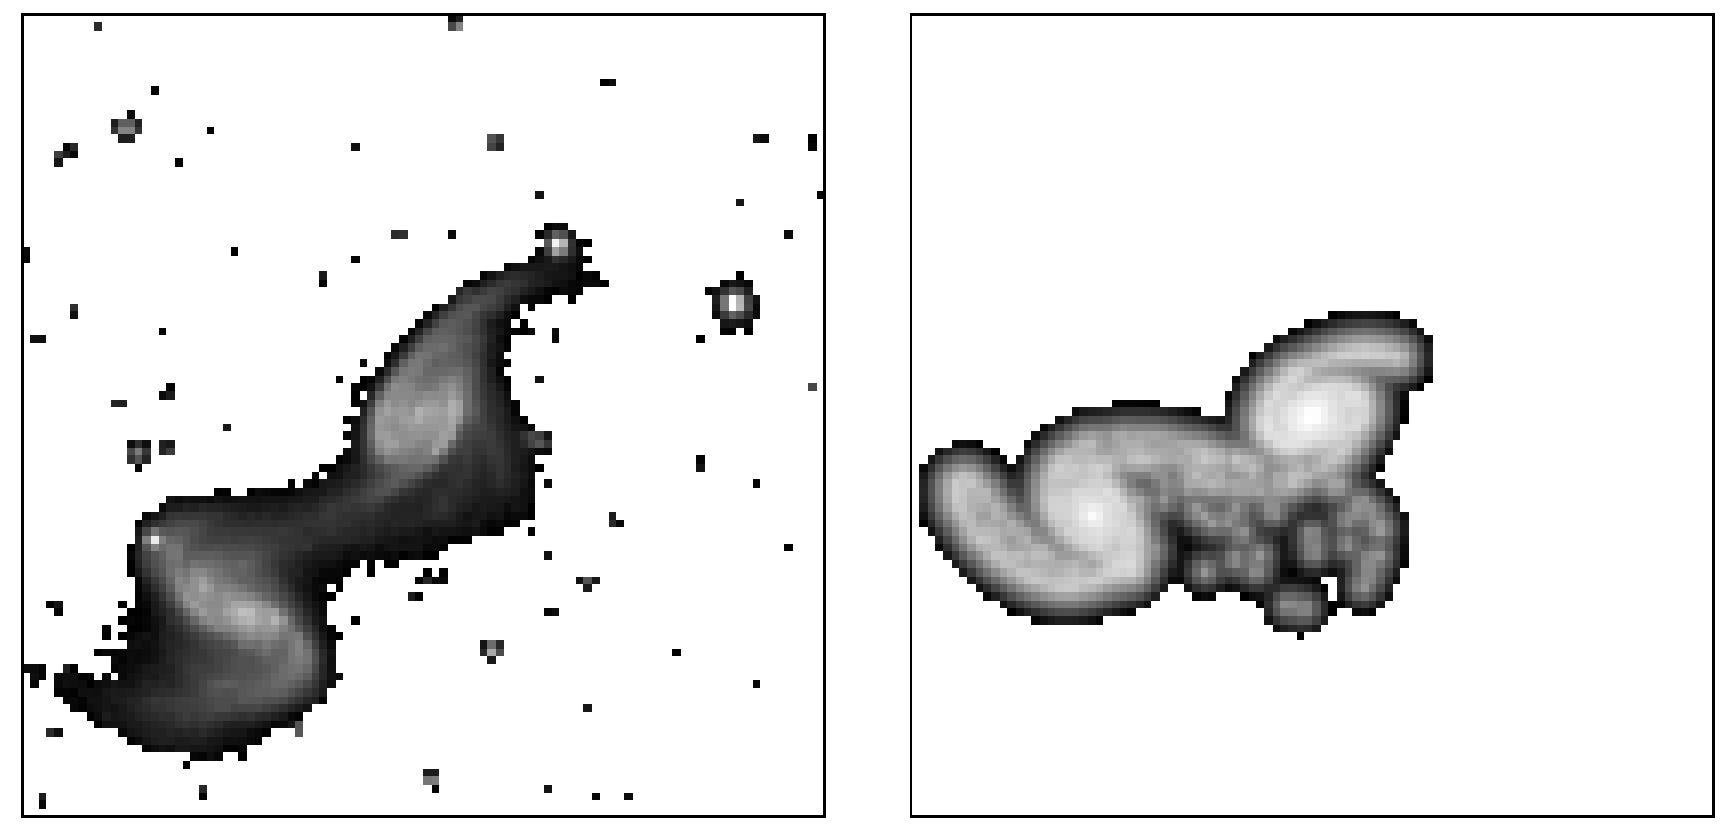
\includegraphics[width=0.75\textwidth]{Chapter1/figures/arp240-obs-sim.pdf}
    \caption{The example system used to test our pipeline: the Arp 240 interacting system. This system is considered an easy one to constrain. It is composed of two clearly distinct galaxies, with strong tidal features that our pipeline can fit. These tidal features are the two tidal tails formed in the interaction and the tidal bridge linking the two systems. \textit{Left}: The prepared observation image of the Arp 240 system created from SDSS DR16 observations. \textit{Right}: The best fit simulation image as found by \citet{Holincheck_16} and the first test image used in our pipeline. The different in scale and orientation are discussed below.}
    \label{fig:arp240}
\end{figure*}

\subsubsection{Simplifying the Likelihood Function}
To further simplify the likelihood function, we can assume our probability distribution is Gaussian. This is a reasonable assumption to make as a starting point for our constraining attempts. However, as will be described in section \ref{Results} this is found to not always hold true; particularly for the orientations of the system. However, making this assumption allows us to utilise the following equation to compare our mock observations to our observed data;
\begin{equation}\label{like_gauss}
    P(D_{obs}|H_{i},C) = (2\pi\sigma^{2}_{j})\exp(-\frac{1}{2\sigma^{2}}\sum_{j=1}^{n}(x_{j}-\mu)^{2}) \times C.
\end{equation}
Here $\sigma_{j}$ is the uncertainty in the observed image, $x_{j}$ is our mock observation and $\mu$ is the observed image. The above expression can be simplified further by noting that the expression in the exponential function is just a half of the $\chi^{2}$ difference between the observational image and the mock observational image. This is the same $\chi^{2}$ function that is used in the code GALFIT \citep{Peng_02}. Where $\chi^{2}$ is given by;
\begin{equation}\label{chi_squared}
    \chi^{2} = \frac{1}{N - n_{dof}}\sum_{0}^{N_{x}}\sum_{0}^{N_{y}}\frac{(p_{x,y} - q_{x,y})^{2}}{\sigma_{x,y}^{2}}.
\end{equation}
Here, N is the number of pixels in the observed image, which has the number of degrees of freedom subtracted from it, n$_{dof}$. $p_{x,y}$ and $q_{x,y}$ are the flux values of the (xth, yth) pixel in the observed and simulated images respectively. $\sigma_{x,y}$ is the sigma value of the (xth,yth) pixel; this is the uncertainty in the observed images pixel value and is the same as that which is defined in GALFIT \citep{Peng_02,2010AJ....139.2097P}. This is then summed over all pixels in the entire image, giving us a single $\chi^{2}$ value between each simulated image and observed image. For now, we define the $\sigma$ image in the same way as described in GALFIT.

Finally, to help computation time the log is taken of our likelihood function. This leaves us with a final expression that a given set of parameters describing a mock observation image also describe the observed image input into the algorithm,
\begin{equation}\label{likelihood}
    \log_{10}(P(H_{i}|D_{obs},C)) = \log_{10}(L) = - \frac{\chi^{2}}{2} + \log_{10}(C).
\end{equation}
This equation is used at every step of our MCMC chain, with a simulation have to be run for each.

\subsection{Architecture for Exploring Parameter Space: \texttt{EMCEE}}
% A short sub-section describing how we set up parameter space exploration in EMCEE.
As stated in the previous section, we utilise the MCMC code \texttt{EMCEE} \citep{Foreman-Mackey_13} to explore parameter space of interaction. For full details of EMCEE and the different modes that it can use, see the extensive readthedocs\footnote{\url{https://emcee.readthedocs.io/en/stable/}}; but here we will briefly state the hyper parameters that we used. 

For each observed image, an ensemble of six hundred walkers was initialised which would explore a total chain length of 7500 steps. Following the advice in the documentation regarding dealing with potentially complex and multi-model parameter spaces we utilised two different walker move proposals in our algorithm. These were the Differential Evolution (DE) Move \citep{Nelson_14} and the Snooker Differential Evolution (DES) Move \citep{ter_Braak_08}. An identical version of our setup can be found on GitHub\footnote{\url{https://github.com/AstroORyan}}. Here, a user can download our setup to reproduce our results, or to update the model for their own purposes.

\section{RESULTS \& DISCUSSION}\label{Results}
\noindent We now apply our described pipeline to the best fit simulations from the Galaxy Zoo: Mergers project. While showing results for every system cannot be done in this paper, they are presented online\footnote{All results are found here: \url{Link_to_results}}. Here, we discuss the constraints on a specific system: the Arp 240 system. We discuss how the constraints could be improved, and what extra information we required for this. We explore the results we find when applying to all simulations, only presenting the results of our three best and our three worst fits, while discussing the trends we see in the remaining results. We briefly present our pipeline applied to observational images. We discuss the limitations of our approach, and how they could be improved upon.

When discussing our pipeline applied to observations, we only look at our best fit subset from applying the pipeline to the best fit simulations of GZM. The computational expense must be significantly increased to make constraints on the observational systems and for our MCMC to reach convergence. We compare our found best fit values and uncertainties to any measured values in the literature, and discuss the difference between applying this to best fit simulations and observations. Finally, we describe the applicability of our approach to other systems; keeping an emphasis on those in the low surface brightness regime.

\subsection{Testing on a Single System: Arp 240}
We apply our automated pipeline to the best fit output simulations of GZM. Specifically, to estimate our performance, we test on the best fit simulation of the Arp 240 system. We elect to use this system as it is is composed of two clear and distinct disks, with a tidal bridge connecting them and tidal tails forming on the opposite side. The tidal features lie in the high surface brightness regime, and have an inclination close to 0. Our prepared observation and the best fit simulation from GZM are shown in Figure \ref{fig:arp240}.

We first apply it to the best fit simulation as this is an excellent noiseless example. This synthetic observation is created with 10,000 particles, and a high time resolution of 0.57Myrs per timestep. We then attempt to constrain this synthetic observation by running the simulation with 2,500 particles with 600 walkers and 7,500 steps in the MCMC. An example of our full results is shown in Figure \ref{fig:corner_plot}. This corner plot is created using the Corner Python Package \citep{corner}.

\begin{figure*}
    \centering
    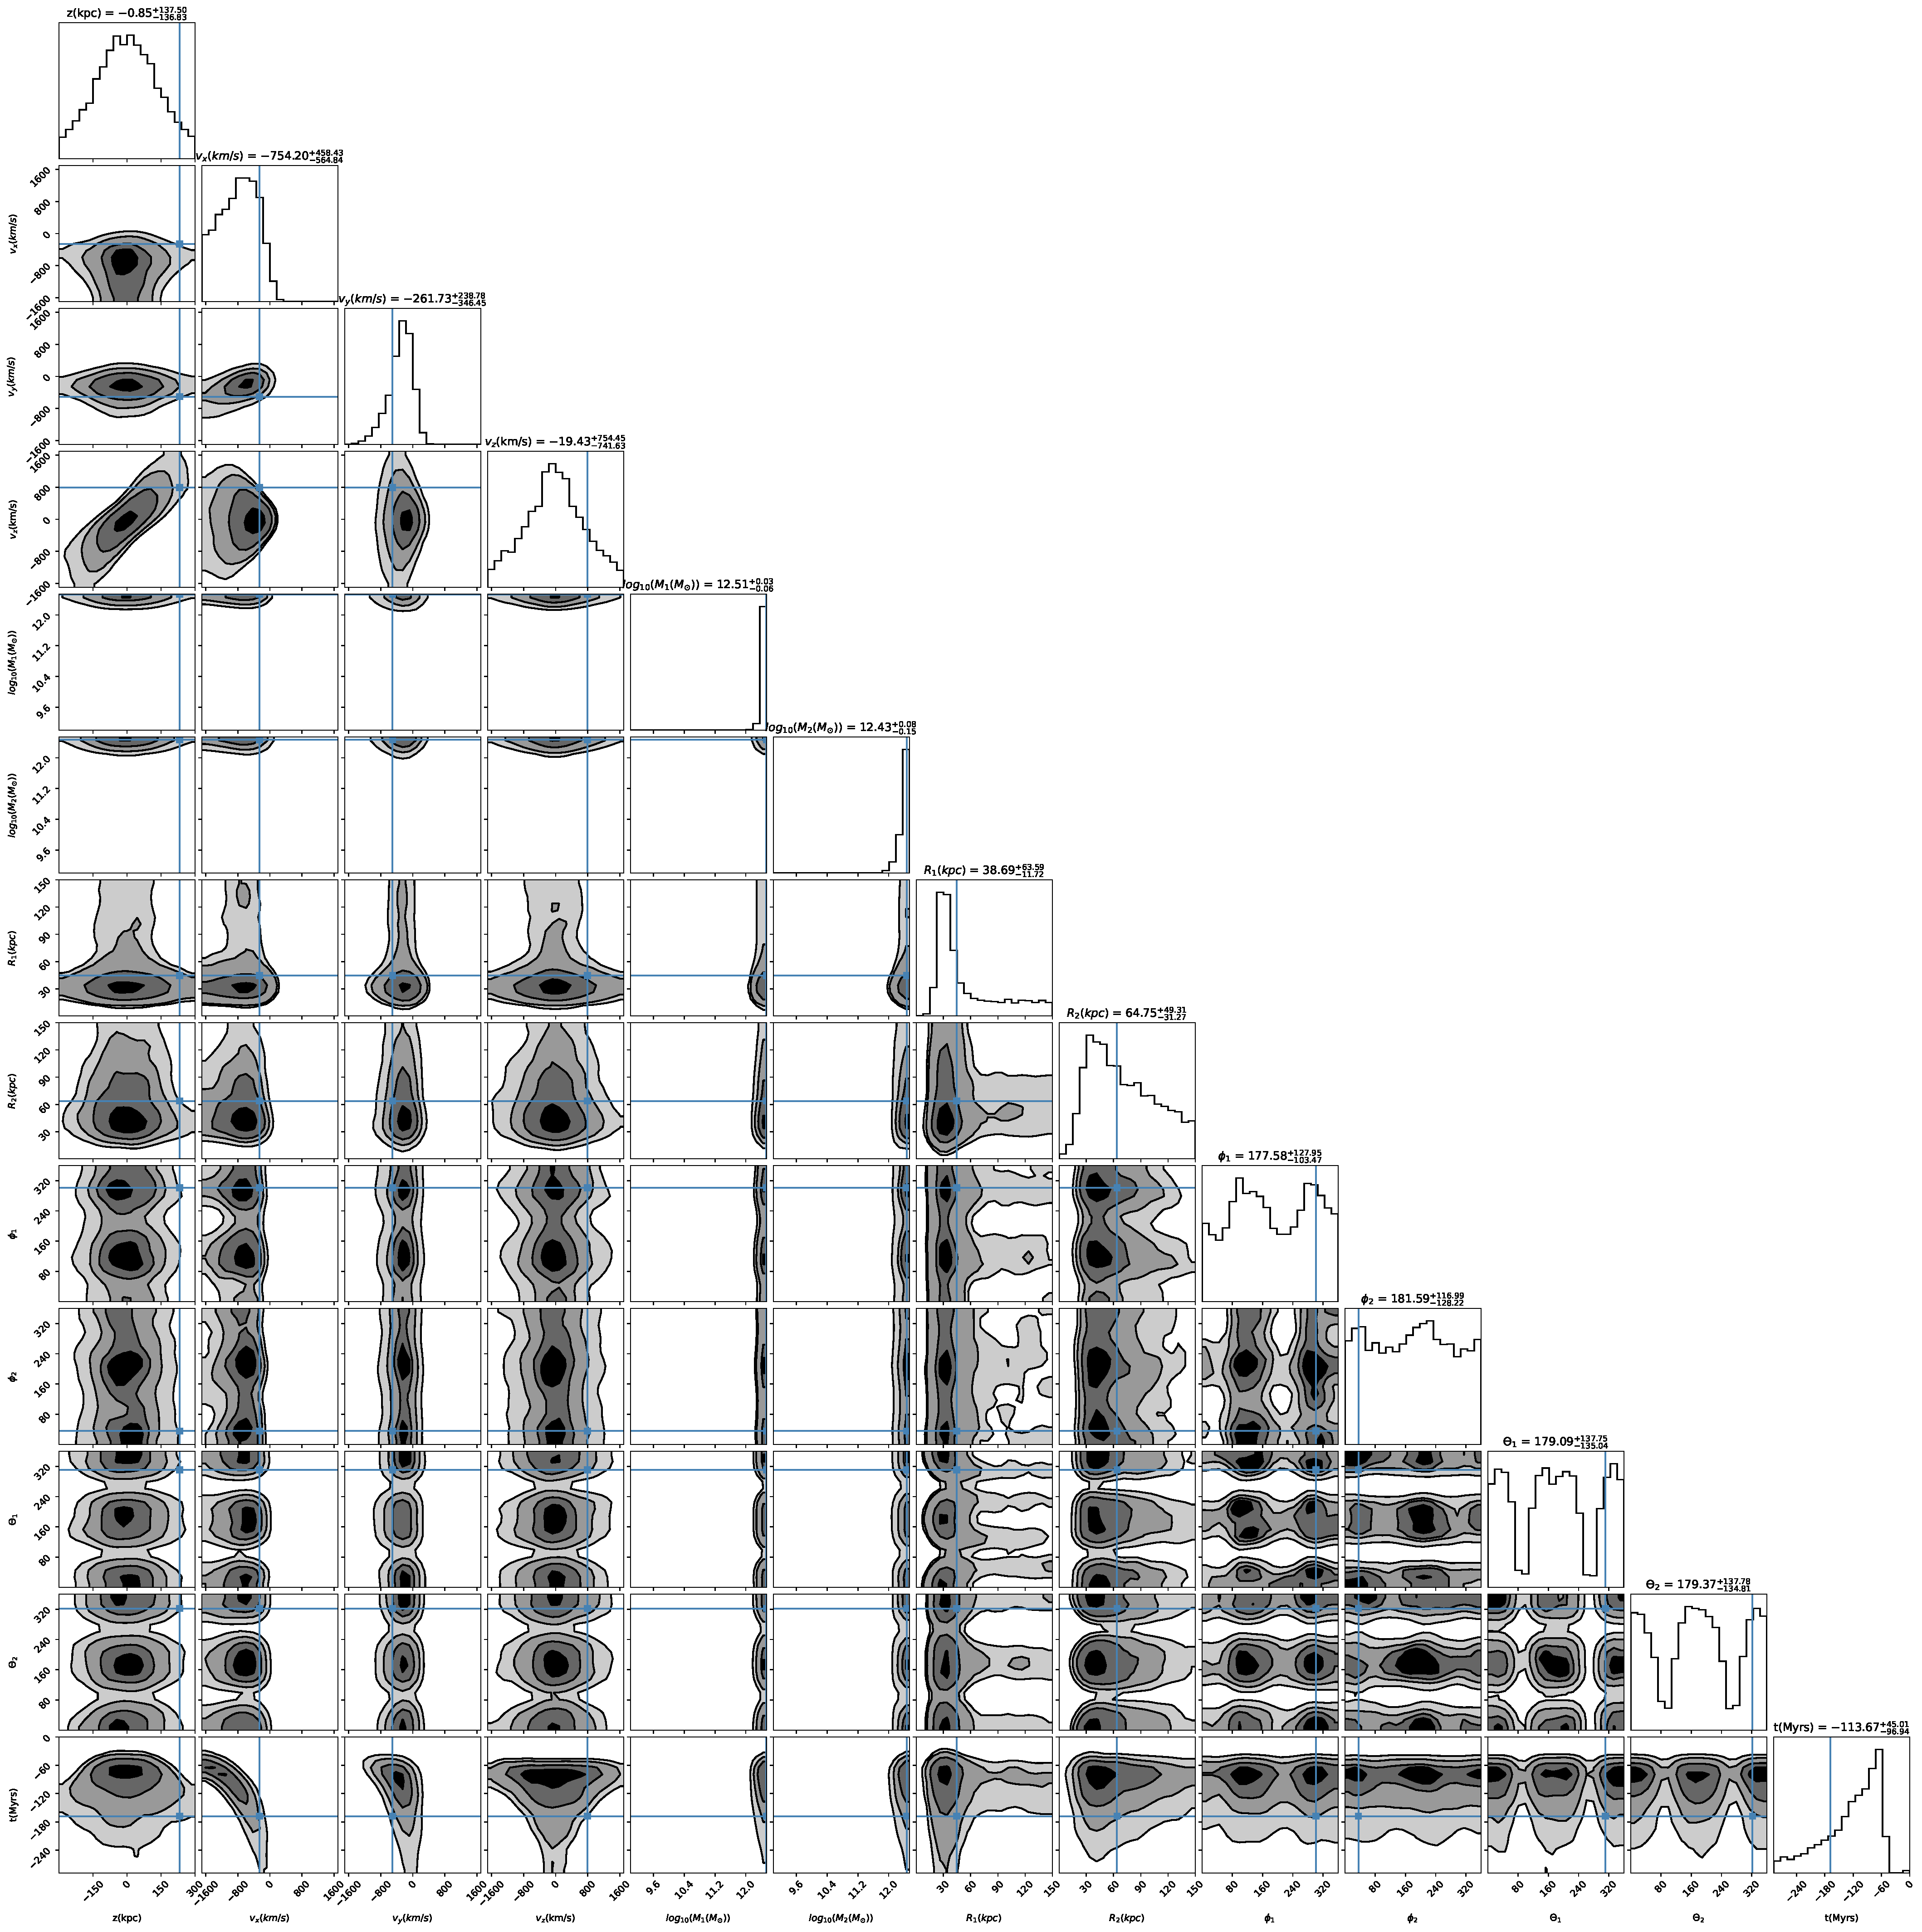
\includegraphics[width=\textwidth]{Chapter1/figures/Arp240.pdf}
    \caption{Corner plot showing the constraints made on all thirteen parameters we are exploring. Contours show the 0.5, 1, 1.5 and 2-sigma levels of the constraint. this corresponds to containing 11.8\%, 39.3\%, 67.5\% and 86.4\% of the samples across all walker chains. Displaying our results using the full corner plot is difficult in a paper because of the high dimensional results that we obtain. Therefore, we elect to show all remaining results in this paper as reduced corner plots like Figure \ref{fig:arp240_corner_plot}. We elect to put the parameters which are most likely to correlate together in different corner plots. To find the full corner plots of each system, find them at the results website for this paper.}
    \label{fig:corner_plot}
\end{figure*}

However, displaying our results as is shown in Figure \ref{fig:corner_plot} will be difficult as we will be discussing multiple different systems throughout this section. This larger corner plot also uses a lot of space displaying corner plots and contours of parameters we do not expect to correlate. Therefore, we will present and discuss our results using reduced corner plots as shown in Figure \ref{fig:arp240_corner_plot}.

\begin{figure*}
    \centering
    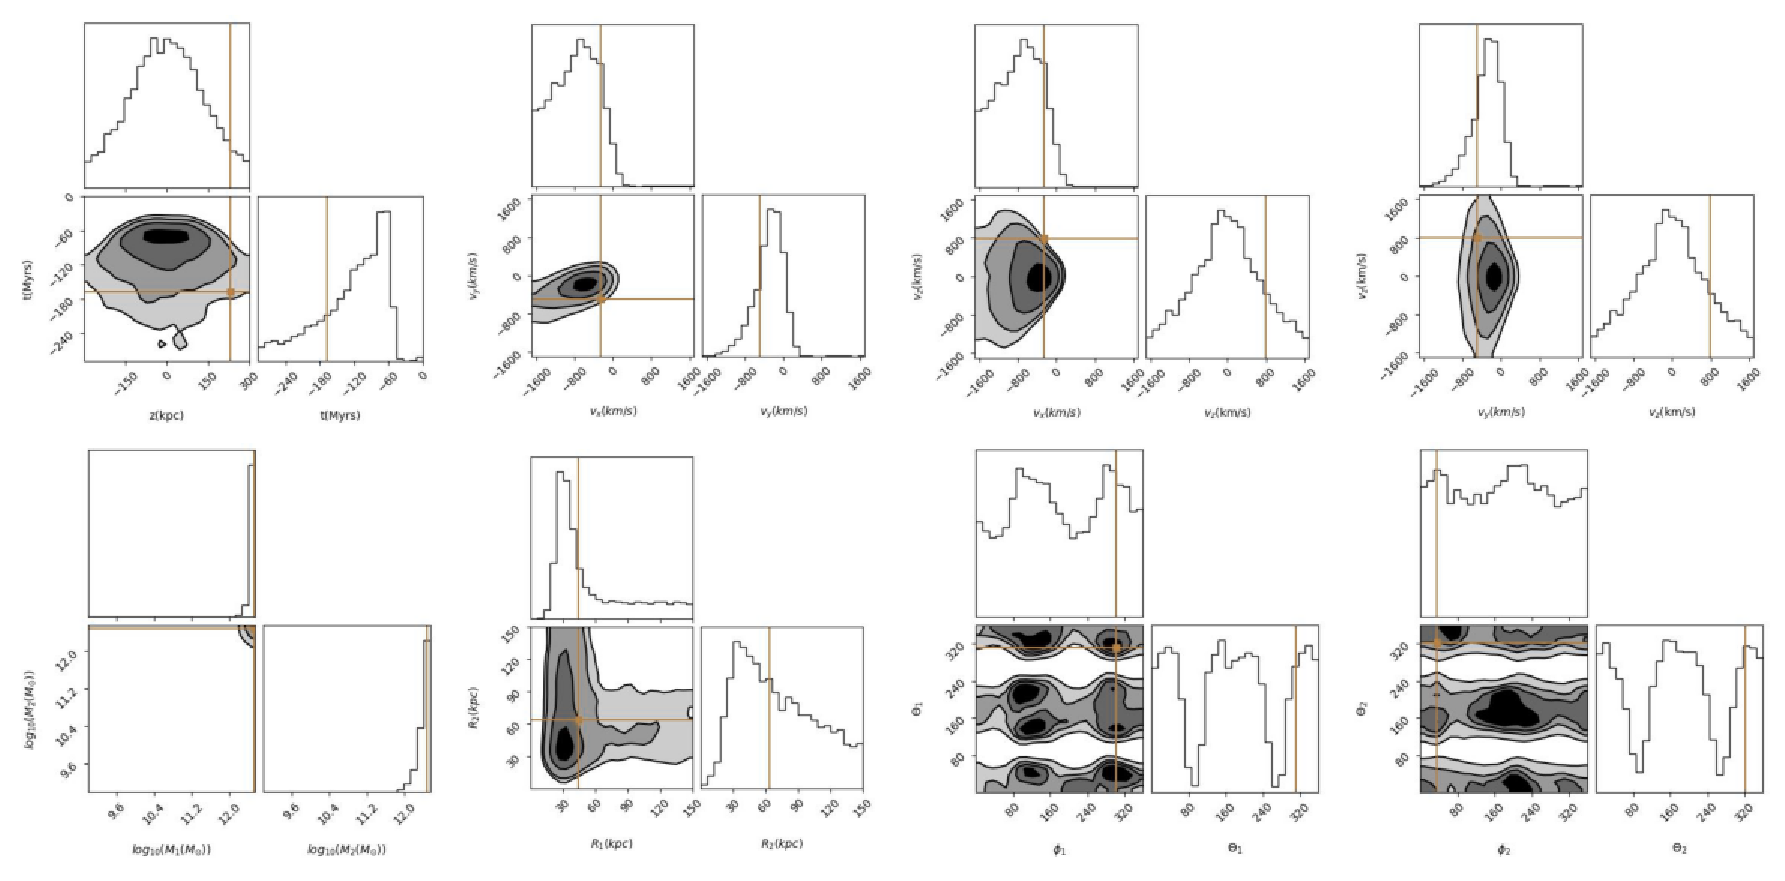
\includegraphics[width=\textwidth]{Chapter1/figures/Arp240-red-corner.pdf}
    \caption{Same as Figure \ref{fig:corner_plot}, but reduced to only matching parameters.}
    \label{fig:arp240_corner_plot}
\end{figure*}

% Describe the results, what are we looking at?
Figure \ref{fig:arp240_corner_plot} shows the constraints we have found on each parameter from our MCMC. The golden lines then show the true values used to create the mock observation. The contours then correspond to 0.5, 1.0, 1.5 and 2-sigma levels (these are default values). Figure \ref{fig:arp240_corner_plot} shows that each of the truth values is within 1-sigma of the peak of the probability distribution with the exception of the z position and time. We also see multiple maxima of probability in the orientation space of the galactic disks.

% Why do the results look like this?
We get excellent constraints on the masses of the two galaxies. The Arp 240 interacting system is the most massive system in our sample, and therefore we expect the mass at the very limits of the range we are exploring. Our pipeline the two masses the easiest to constrain out of all the parameters, and this is the first parameter which converges in the MCMC. We provide the algorithm with the secondary two dimensional position, and therefore it has to only fit the flux distribution of the inner disk correctly to get good constraints on the galactic masses. It knows where to place the secondary and then just has to match the pixels on the inner parts of the galaxy to quickly increase the likelihood. While the formation of the tidal features is dependent on the mass ratio, we have found that they are also very dependent upon the orientation of the interaction as well as the relative sizes.

We can see that the relative sizes of the disks is important for the constrainingt he tidal features as there is a very large spread in the constrains. The primary radius is constrained very well, and is primarily expected to be smaller than the true value of this system. This is, again, due to the $\chi^{2}$ nature of calculating the distance between the two images. The likelihood, on average, is lower with some pixels within the galaxy being missed than a pixel containing galaxy in it when it shouldn't. We therefore have a bias effect where the peak of probability drifts towards just below the true value of the radius. However, the true value of the radius remains within 0.5-sigma of the found contours, and therefore this acts as a good approximation. 

The secondary galaxy has significantly larger uncertainty of its radius. The large tail in the 1$\sigma$ in the marginalisation shows this. This is from a limitation of our simulation as well. While the output simulations of the MCMC are always centred on the priamry, the secondary galaxy central position is not so certain. Due to the backwards integration and trajectory calculated here, the secondary does not always end in the exact same image bin in the output simulation image. Therefore, the secondary disk likely moves slightly per simulation (by $\pm$1 bin in the x or y direction). This change transfers further uncertainty in the secondary disk size. However, once again, the best fit values found are within 1$\sigma$ of the true value from the base simulation. 

There will also be some uncertainty involved in this measurement from the formation of the tidal features. The flux distribution of the tidal features that form are inter-dependent on multiple parameters; primarily the mass ratio, the size ratio and the orientation of the galaxies in the interaction. The significant degeneracy in the orientation constraints undoubtedly has some effect on the fitness of the resultant system. Due to a lack of three dimensional information, our algorithm cannot discern which way the galaxy is rotating or which way the tidal features should be orientated in the line-of-sight. Therefore, degeneracy at $\pm180^{\circ}$ of the true parameter values for $\phi$ and $\pm$180$^{\circ}$ for $\theta$. Figure \ref{fig:arp240_corner_plot} shows this with several different peaks in both measurements of $\phi$ and $\theta$.

It is important to note here that $\phi$, in our simulation, is the orientation of the galactic disk with respect to the y-plane while $\theta$ is the orientation with respect to the z-plane. With three dimensional information, such as the direction of rotation of the disks or the line of sight (LOS) velocities of the tidal features, we would be able to resolve the degeneracy in the $\phi$ parameter. However, The source of the degeneracy in $\theta$ has a different source. The tidal features can actually form in the opposite direction from the mock observation and still be found to have high likelihood. This is a result of our likelihood being based on flux matching on pixels. There is no knowledge provided of the direction the tidal features should be moving or forming, only if the pixels contain the correct flux. Therefore, this gives a significant degeneracy in the $\theta$ parameter. Therefore, while the disk can be flipped in the z-direction and still match the observation, it can also be flipped in the y-direction as well. While the degeneracy in $\phi$ can be solved with velocity information, a more subtle approach will be needed to solve the degeneracy in $\theta$.

The lack of three dimensional information also affects out constraints in the z-direction: the z-position and the z-velocity. As seen in Figure \ref{fig:arp240_corner_plot}, the algorithm fails to constrain the z-position, while there is significant uncertainty in the z-velocity. First, the z-position is difficult to constrain as we lack three dimensional information. The simulation is run in the reference plane of the primary galaxy, therefore the secondary can only be behind or in front of the primary galaxy. There will be change in the flux of the secondary based on whether it is in front or behind of the primary galaxy. However, this change in flux is completely dominated by the distance due to the redshift of the galaxy. Therefore, there is little to no observable change in the absolute values of flux unless the true value of the z-position was very large.

The z-velocity remains largely unconstrained due to similar reasons as above. The true value lies at the very edge of the probability distribution found, at approximately 2$\sigma$. This would, again, be rectified readily by introducing velocity information into our constraints. The simulation works so that the secondary galaxy always is at the same x and y position that is defined by the user (or calculated from the observation). Therefore, an output simulation with a positive or negative LOS will have the same flux distribution. Hence, this constraint simply peaks about zero for the z-velocity.

Our pipeline works significantly better, however, with the x- and y-velocity of the secondary galaxy. We find the the truth value of this is within 1$\sigma$ of our found distribution. The velocity values are directly related to the strength of the interaction, and therefore indirectly relate to the tidal features which form. Thus, our pipeline is informed by the flux distribution of the resultant and gives an excellent constraint on the parameters.

% Need to replace this time of interaction with the correct one. 
Finally, we discuss the attempting to constrain the time of the interaction. Shown here is not the total time of the interaction, but how long ago the time of closest approach was. The underlying simulation utilises backwards integration to calculate the trajectory of the interaction. Therefore, the time we input into the simulation simply tells it how far back in said trajectory to put the secondary galaxy. Therefore, the same interaction will occur whether we input -10 time units or -100 time units, the algorithm will require more computation time calculating the particle positions in the lead up to the interaction. It is important to note that the total integration time will only affect the output system when we make it too small. I.e., if the secondary starts after the point of closest separation or at closest separation, our simulation breaks down and gives nonphysical results.

We calculate the time of closest approach for all of our walker steps and then present this as a measure of the time posterior distribution. Our measured value is significantly smaller than the true value of our best fit simulation, although it does lie within the region of 2$\sigma$. This parameter is highly dependent on the velocity and position constraints that we have made, and these are skewed to significantly smaller values than the truth. Therefore, it is unsurprising that our time of closest approach value is also found to be much smaller.

To fully put this result into context, we explore the simulations that lie in the areas of highest probability within these posteriors. To select which simulations to present, we take those walkers that had the highest log probabilities throughout each walker chain and take the top 5 as an illustration here. What we find is that our pipeline is not able to precisely reproduce the best fit simulation from GZM. It is often able to reproduce the tidal features of the primary as well as the tidal bridge connecting the two systems. This appears to be where the pipeline has centered the posterior upon. The likely reason for this is actually due to the filtering parameter that we use on the simulation. The Arp 240 simulation lies in an unlikely area of tidal features to form - $\gamma = 0.259$ - and, therefore, we update our prior to make the true result appear less likely. However, the $\gamma$ parameter remains a necessity in our constraint pipeline. Without the ability to filter the simulations quickly, the parameter space is simply too large to fully explore in a computationally reasonable time. Therefore, for this particular example the $\gamma$ parameter is a hindrance.

\begin{figure*}
    \centering
    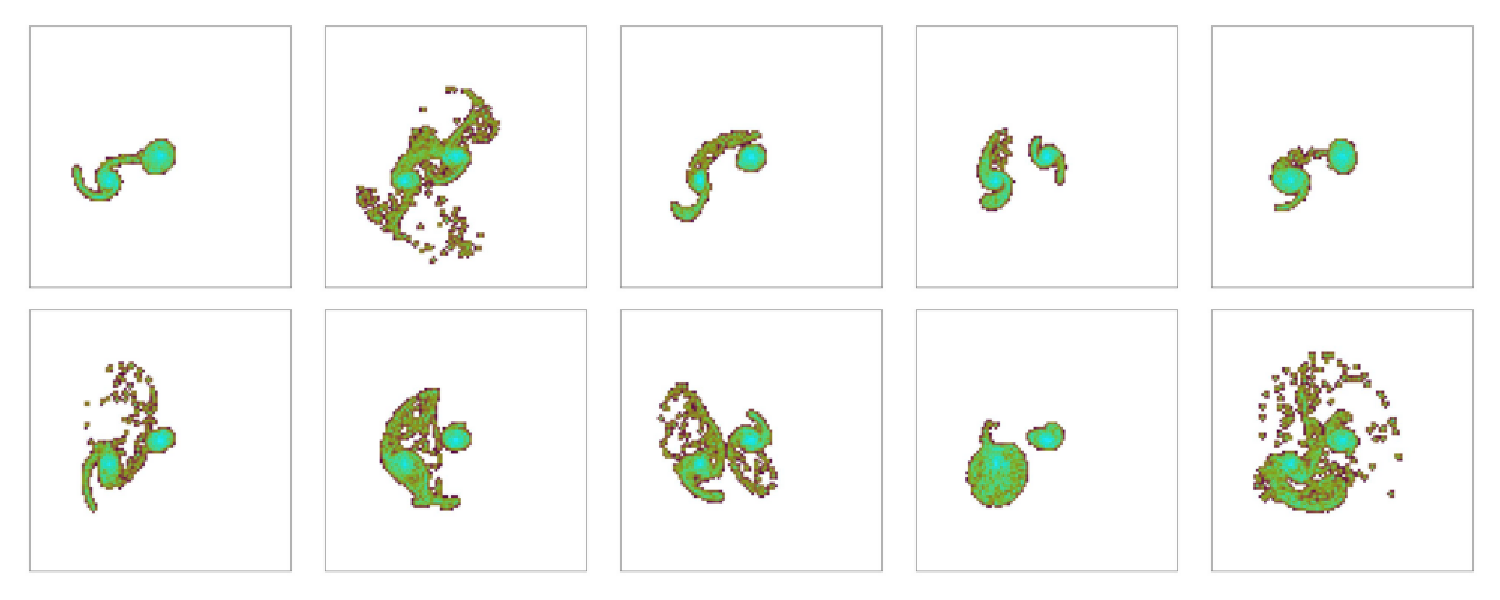
\includegraphics[width=\textwidth]{Chapter1/figures/best-fits-comb.pdf}
    \caption{Simulations from the areas of parameter space that lay within the 0.5$\sigma$ of our constraints. \textit{Top}: The best fit simulations from this parameter space. \textit{Bottom}: The worst fit simulations from this parameter space. Our pipeline has found those parameters which cause the formation of the correct tidal features, as well as the tidal bridge connecting the two systems. However, it has been unable to fully identify the tidal features of the secondary. There is also a lot of noise in this posterior distribution, with many systems with wildly different tidal features in the areas of high probability. Therefore, identifying specific systems with the sought after tidal features remains needing to be a manual process.}
    \label{fig:arp240_corner_plot}
\end{figure*}

% This is likely better in the conclusion.
In the surrounding area of probability space, however, we find some interesting results. Changing each parameter by some amount based on the posteriors of each parameter space leads to variation in the simulation outputs and tidal features. Due to the disks being well defined and aligned, this can often lead to them being weighted highly. Therefore, the question remains, how would one use this code to find their best fit simulation and actually make constraints using it? This algorithm is best used as an indication of where in parameter space the true parameters lie in recreating the tidal features observed in an observation. This reduces the size of parameter space to explore dramatically, and could be an indication of where to search with more accurate simulation models for true interacting galaxy parameters.

Overall, from our example of Arp 240, we are able to recover nearly all the true values of the input simulation to within 2$\sigma$ of the true parameters. The only missing parameter is in the secondary $\phi$ parameter. There is significant degeneracy in constraining the orientations of this interaction, but this is not unexpected. While our results appear like they have converged in the MCMC, we will also describe the diagnostics with which to prove this. 

\subsection{Diagnostics of Pipeline}
% Note, a quick section to discuss the diagnostics of the pipeline, proved it's converged etc. If I cannot get Chain Consumer working here, then I won't do this section.
\noindent It is important to ensure our results are reliable by using diagnostics to investigate the MCMC chains. We investigate three different diagnostics of our MCMC run. First, we check that they have truly converged with the Geweke diagnostic. The Geweke diagnostic is a Z-test of equality of means where the autocorrelation in the flattened samples is taken into account as the standard error is measured. We use the Geweke diagnostic as written in the ChainConsumer \citep{Hinton2016} Python package. For this case, every parameter passes this convergence test, with the exception of the orientation parameters.

Figure \ref{fig:arp240_corner_plot} clearly shows that $\phi_{2}$ has not converged, given the marginalised posterior is has very limited structure with two insignificant peaks. With the remaining three orientation measures, this is more complicated. Here, we have a two or even four fold degeneracy in the output models due to three dimensional information not being available. This disrupts our Gewke diagnostic measure, which is looking for a single peak in parameter space. Therefore, by folding the parameter space over and only exploring over $0^{\circ}$ - $180^{\circ}$, we achieve a single peak in parameter space. These remaining three results then pass the Geweke diagnostic test. The failure of $\phi_{2}$ to pass the Geweke test means that more steps in each chain must be run to reach true convergence.

\begin{figure}
    \centering
    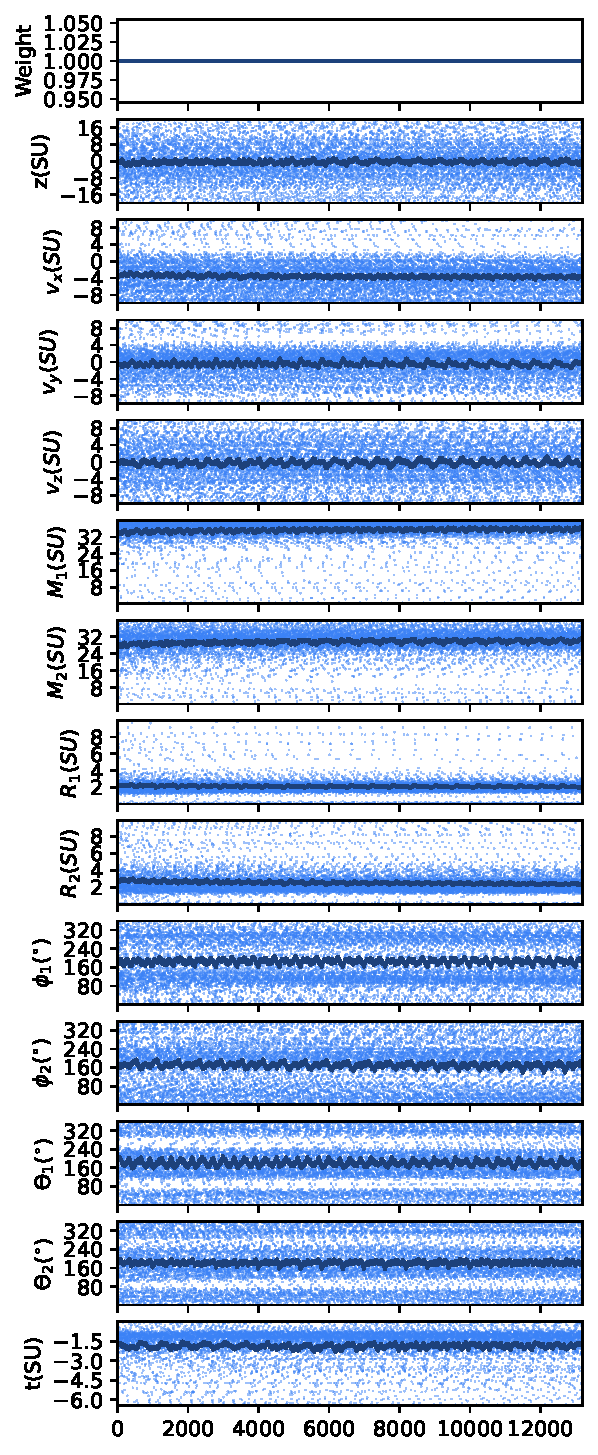
\includegraphics[width=0.45\textwidth]{Chapter1/figures/arp-240-steps.pdf}
    \caption{Steps taken by each walker in our MCMC chain to constrain the Arp 240 best fit simulation. Note, the y-scales here do not extend over the full parmaeter space for some galaxies, and only show where the walkers have stepped after the burn-in phase. The deeper the blue, the more walkers have stepped at that point. This figure shows that our MCMC has successfully burnt in and very quickly goes to high areas of probability for parameter space. They then oscillate around the best fit values while searching the remaining parameter space. The z, z-velocity and $\phi_{2}$ parameters show dignificant uncertainty as the walkers move around the entire parameter space. In the $\phi_{1}, \theta_{1}, \theta_{2}$, we can see the two fold degeneracy form very early on and then the walkers do not explore across them at any point.}
    \label{fig:walker_steps}
\end{figure}

The second diagnostic we check is that the walkers have fully explore parameter space and that we have removed enough of the steps at the beginning of the run to consider the MCMC burnt-in. Once again, using ChainConsumer, we can plot out each walker step throughout parameter space. Figure \ref{fig:walker_steps} shows the flattened walker chains through parameter space. We have removed the first 200 steps of each walker chain before thinning the chain and flattening it. By flattening we have taken each walker chain and combined them into one chain for every parameter. Simply discarding the first 200 steps has been enough for the burn in of the MCMC, as the walkers have already moved mostly through parameter space and are centering on a central value of high probability. The structure in the orientation parameters is also interesting. The degeneracy structure in the parameter space has already formed by the end of the burn-in and then the walkers move within those areas of high probability. This is for two reasons. First, as stated previously, the orientations do not have a massive impact on the flux distribution of the disks of the output interacting system. The Arp 240 interacting system is face on, and therefore the degeneracies form where the disks are face on and the empty areas are where they would be edge on. Second, when they are in that degenerate space, the slight changes in inclination of the disks given does not change the likelihood calculation significantly enough to reduce this degenerate space further. Hence, the degenerate areas are very large with very flat areas of probability at their peak.

We have tested resolving this problem by running further steps in our MCMC to achieve convergence naturally within the parameter space. We find that increasing the number of steps does improve convergence on the orientation parameters, but at the cost of little improvement for the remaining parameters. This is also at the cost of much larger computational expense. Therefore, we elect to fold our resultant degenerate solutions into a smaller parameter space. This achieves convergence, and gives us excellent estimates on the orientation for these systems.

A second solution to this problem would be involving velocity information into our models. Knowing the bulk motion of the tidal features would allow us to constrain the tidal features based on which way they were rotating. This would eliminate part of the degenerate space. However, as stated previously, little spectroscopic data exists of the GZM sample galaxies. Therefore, we run this test using the same best-fit simulation but taking the LOS velocity of the particles and creating a velocity grid to constrain over.

\subsection{Inputting 3D Information}
Very few of the systems in the GZM sample have associated IFU data in order to get LOS velocities to incorporate 3D information into our fitting pipeline. Therefore, we once again test incorporating these by using them with a best fit simulation of Arp 240. From these, we simply sum the z-velocities of each particle in the bin and then create a total LOS velocity map for which to compare to simulations. This has little impact on the measurements of mass, size and x- and y- velocity measurements. However, it completely changes our measurements of the z-position and allowed us to completely constrain the z-velocity. 

Figure \ref{fig:velocity_corner_plot} shows the new measurements of the constraint on the z-position, y- and z- velocities. We can immediately see that the constraints on each of these parameters is significantly improved. This is with the same number of MCMC walkers and steps remaining the same from running without. For the y- and z- velocities, the constraints are improved to the point where we completely recover the true underlying parameter values within 0.5$\sigma$. With the z-position, we also gain significant constraint. The pipeline is able to recover which side of the primary the secondary lies, with a sharp drop in the marginalised posterior over the negative part of the z-position parameter space.

\begin{figure*}
    \centering
    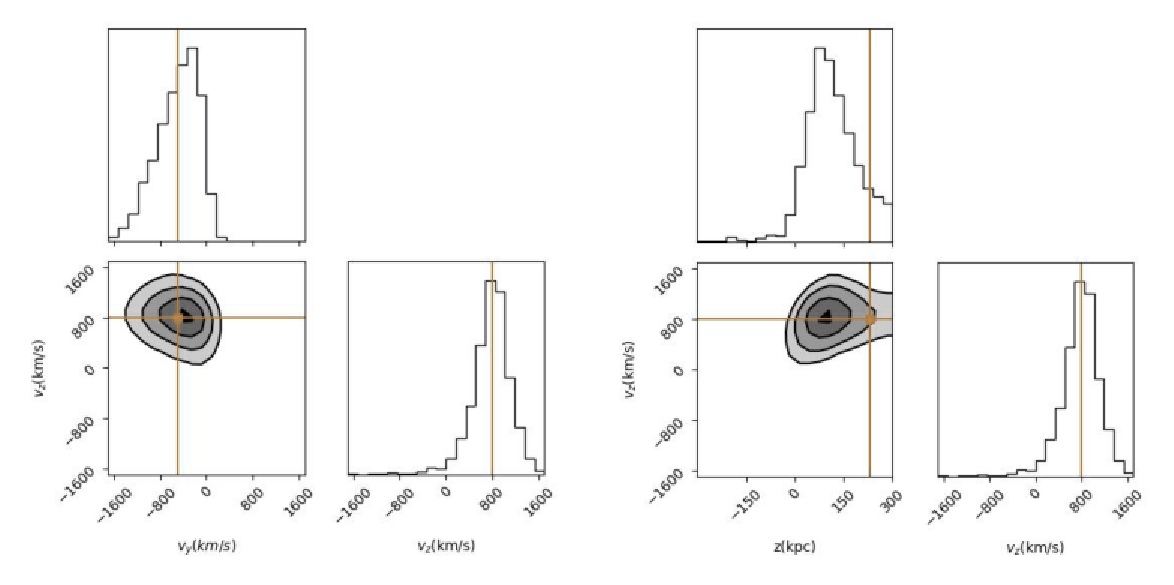
\includegraphics[width=0.9\textwidth]{Chapter1/figures/vel-red-corner.pdf}
    \caption{The constraints on the 3D velocity and z-position when including velocity in our MCMC pipeline. To add this extra information, we ran our best fit simulation of Arp 240 and summed the LOS velocity (z-velocity) in each pixel of our image. Comparing between here and Figure \ref{fig:arp240_corner_plot}, we can see that we achieve complete constraint of the z-velocity of the interacting galaxy. We also significantly improve the constraint on the z-position parameter as the pipeline is able to distinguish which side the secondary galaxy is of the primary.}
    \label{fig:velocity_corner_plot}
\end{figure*}

Other parameters are not shown in Figure \ref{fig:velocity_corner_plot} as there was no change in their constraint after adding in velocity information. This was unexpected with the orientation constraints of the galaxies. However, it is important to note that, in this example, we have only used the LOS velocities to achieve this improvement in constraint. To better get constraint on orientation, we likely would need higher resolution on our velocity map than the simple 100 $\times$ 100 binning we used. We would also need further information about the rotation, and get accurate measures of the bulk motion of the tidal features in the galaxy. Currently, the simulation is not able to accurately reproduce this outwith simply assuming circular velocities at different radii from each galactic centre. 

This shows the improvement that adding velocity information to our methodology could bring, and how far interacting galaxy simulation and constraint can go once we incorporate integral field unit (IFU) spectroscopy over more systems. In the sample we are using here, of the most massive, large, major interacting systems, only three have got any IFU data. This data is from the MaNGA \citep{2015ApJ...798....7B} IFU spectrograph, whose field of view is only able to capture the central disk of these systems. To significantly improve our constraints, we will need this information of the tidal features of these systems. IFUs with larger fields of view are soon to come online, such as WEAVE \citep{2014SPIE.9147E..0LD}. When this does, we will be able to fully apply the velocity and rotation information of these systems to this methodology, and reach a true conclusion of the improvement we could reach.

\subsection{Recovering the Galaxy Zoo: Mergers Results}
% Remember, this section is meant to be an overview of all of the results and simply a discussion on what we notice of applying it to different systems. This is not another deep dive like we did in the testing on one system. 
\noindent With constraints being ascertained on nearly all parameters of Arp 240, we then applied our pipeline to the remaining 61 interacting galaxy systems of the Galaxy Zoo: Mergers sample. The reader is invited to see the resultant corner and reduced corner plots of each system on the website. Here, we will detail observations and trends from applying our pipeline to multiple systems. First, our ability to make constraint is highly dependent upon the stage of interaction. Our tightest constraints, the ones with narrowest posteriors, were on those interacting galaxies which were only just past the point of closest approach. I.e., they were the systems which had highly distinct tidal features and disks were fully separate. Our best three fits were those of Arp 172, Arp 240 and Arp 290. The `best fits' have been judged by those with the smallest FWHM of their marginalised probability distribution in mass. This constraint on our three best fit and three worst fit systems are shown in Figure \ref{fig:mass_constraint}.

\begin{figure*}
    \centering
    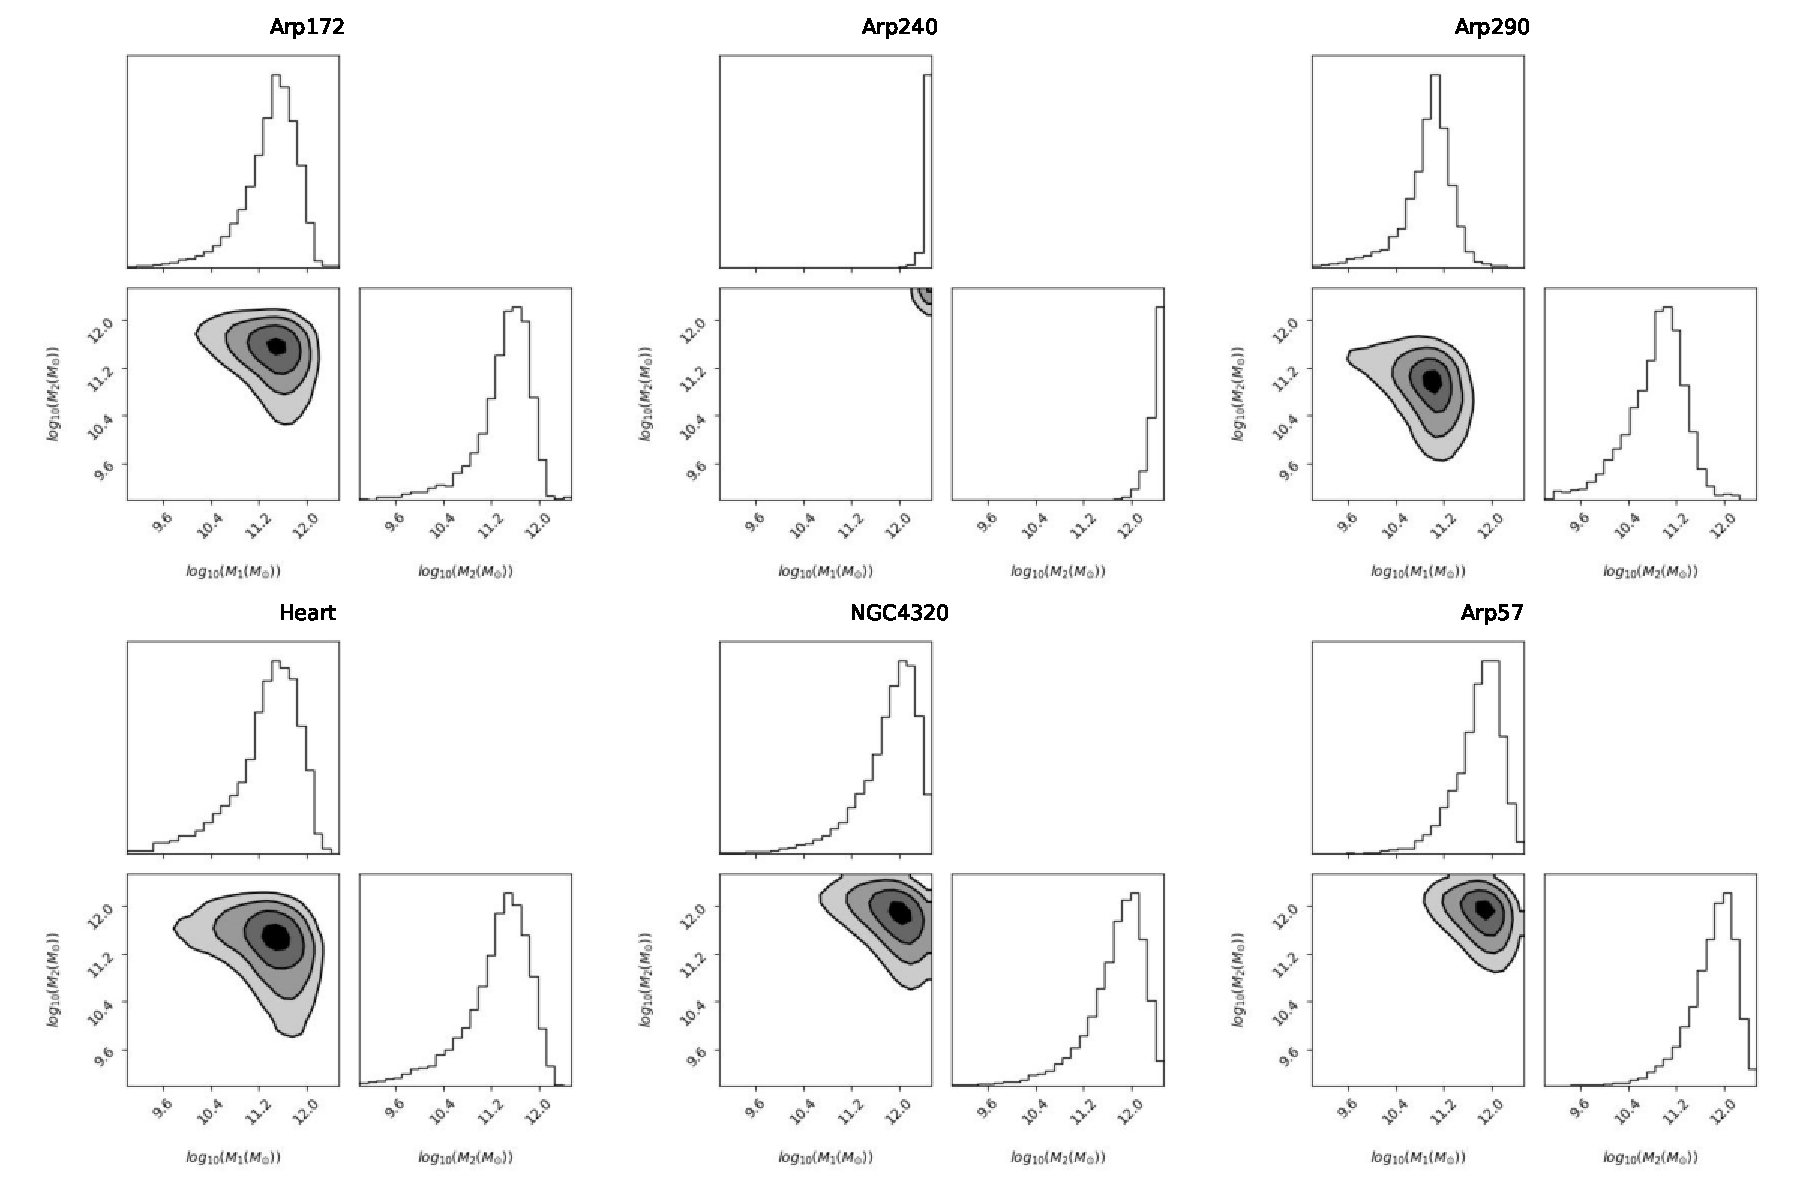
\includegraphics[width=0.9\textwidth]{Chapter1/figures/masses-comb.pdf}
    \caption{Mass corner plots for our best and worst fits from the pipeline. This was judged by the FWHM of the marginalised posteriors. \textit{Top}: Our top three best fits. \textit{Bottom}: Our worst fits. Even with our worst fits here, the masses are very well constrained.}
    \label{fig:mass_constraint}
\end{figure*}

The worst fits we achieved were of those systems which were close to the merging stage. They were systems where the two cores were close to coalescence, very little tidal features were visible or the position of the secondary galaxy was very unclear. Our worst three fits and examples of this were Heart, NGC4320 and Arp 57. Each of these systems represent these three limitations, respectively. It is relatively easy to see why these limitations lead to difficulty in our pipeline. If two cores are close to coalescence, the flux distribution will appear similar to two overlapping disks. Therefore, our pipeline will calculate equivalent likelihoods between systems with little to no interaction and a merger with multiple flybys undergoing coalescence. Our pipeline is also not yet designed to account for multiple flybys, a key assumption being that these systems are only on their first passage. Our pipeline requires tidal features to make fits on the flux distribution. NGC 4320 is a system where we have reduced the resolution so much that we lose spatial resolution in the flux distribution of the tidal features. Therefore, we insert a significantly higher uncertainty into our constraints. Finally, our pipeline requires a secondary galaxy to make reasonable constraints on the underlying parameters. The example of NGC 4320 is a final stage merger where a large tidal feature has formed as a result of the coalescence. While our pipeline is able to reproduce the tidal feature, it is unable to reproduce the flux distribution as found in the original Galaxy Zoo: Mergers project.

% Now, going to break down the generals about each parameter space.
Throughout every system we put constraint on, the parameter we are able to get reliable constraints on are the masses of the systems. This is shown above as even our worst fit systems still hold excellent constraints, with the values confined to small areas of parameter space. For every single system, the worst fit parameters were the four orientation parameters for the two galaxies. Aside from the points that have already been raised regarding the problems of our pipeline constraining these, a further problem was that the likelihood calculation is dominated by contributions from the mass and velocity parameters. As long as the shape of the final system is correct, the orientations only alter the likelihood by between 0 - 20 points. Whereas the mass can be the difference in hundreds. There are solutions to this, however. Further walkers and a longer chain can be run to strengthen these constraints, but this comes at the cost of far more computational expense. Second, only a subset of the orientation space could be explored. Due to the 2- to 4- fold degeneracy in the orientations, only a small section of the orientation parameter space needs to be explored. For the purposes of this work, we show the full degeneracy and what is to be expected throughout all of the parameter space.

\begin{table}[]
    \centering
    \begin{tabular}{c|c}
         &  \\
         & 
    \end{tabular}
    \caption{NOTE: To be added as the MCMC runs finish. Or, may go online! Actually, likely to be a machine-readable table.}
    \label{tab:constraints}
\end{table}

% A word about marginalising over all posteriors?
The remaining parameters, and their level of constraint, lie between our best case scenario of the mass constraint and the worst case scenario of the orientation constraint. However, the importance here is that we are able to reproduce the Galaxy Zoo: Merger best fit values and uncertainty measures without the need for human interaction. Thus, this pipeline and methodology can be applied to larger samples of galaxies than we have presented here. Table \ref{tab:constraints} gives a full breakdown of our results for each system. This includes the best fit value for each parameter from the MCMC runs as well as the errors upon them. Comparing with the GZM best fit results (as an accompanying machine readable table), shows where improvement is needed but also that for nearly all parameters are pipeline is successful. 

The true power of this approach will be when investigating large populations of interacting galaxies and combining and marginalising over many different posteriors. When combining the parameter spaces of many different systems, it will be possible to identify those areas of parameter space which lead to the formation of certain features across populations of interacting galaxies. Our method will allow more intense simulations to sample smaller parameter spaces and be more efficient when finding systems with specific features. However, how to combine the posteriors is somewhat up for debate. We have ensured that the parameter spaces we are exploring are equivalent in size and that the prior is equal across parameter space. There thus comes the question of the $\beta$ parameter in filtering simulations which, indirectly, changes the prior based on the trajectory of the interacting system. To conduct this combination, we would recommend that the $\beta$ parameter was not utilised when building the different posteriors. However, this will come at an increased computational cost. 

However, all of our results so far have been in the best-case scenario of a noiseless best fit simulation. The translation from simulation to observation in pipelines such as these is never an easy one. We, therefore, use the our top three best fit systems here (Arp 172, Arp 240 and Arp 290) and apply our pipeline to their reduced observations.

\subsection{Applying to Observations}
% Brief re-iteration of creating observations.
\noindent We apply our pipeline to the reduced observational data of Arp 172, Arp 240 and Arp 290. Cutouts were created as described in Section \ref{Methods}. We reiterate here that the cutout resolution is reduced from its native resolution to images of 100 $\times$ 100 pixels. Before we input the images into the pipeline, we find the central pixel of the secondary galaxy and convert this into a physical x- and y-position. We also find the total size physical size of the cutout in kpc, convert it to simulation units and provide this to the pipeline. We find that the physical size of the cutouts are significantly different from the cutout sizes used by GZM in their work. As an example, we create the cutout of Arp 240 at 600 $\times$ 600 pixels at native resolution. With SDSS data, this corresponds to a physical size of 111.50kpc $\times$ 111.50kpc at the redshift of Arp 240. The best fit simulation from GZM for Arp 240 is 785.35kpc $\times$ 785.35kpc. Figure \ref{fig:arp240} clearly shows a very different scaling between the observation and simulation, however, it is not enough to be seven times zoomed in on the system. We also find that the secondary positions are very different between the observation image and that used in GZM. As a result, the parameters we will find for constraining the observation will be very different from the values found in GZM. 

% Why do we take significantly longer on these?
We apply our pipeline to our three best fit simulations. We only investigate these three systems as we find the computational expense is significantly higher when constraining the observations compared to the best fit simulations. We find the reasons for these are two fold. First, we must run each walker for twice the number of steps than when constraining the best fit simulation to reach convergence. Second, due to the smaller scale size of our images, the defined $\gamma$ parameter is much stronger than with the GZM sample. Both of these reasons for higher computational expense are to be expected. We are now constraining over images with noise, rather than the noiseless images of the best fit simulations. The increase in the $\gamma$ parameter also means that we are filtering out less candidate systems and running the base simulation code more often. This directly translates into a higher runtime for our pipeline.

% What do we find immediately?
Figure \ref{fig:obs_corner_plot} shows the reduced corner plot for the observed Arp 240 system. The constraints on the velocity parameter have significantly worsened when compared to the constrains on the best fit simulation. They are also in a different area of parameter space when compared. The velocity and spatial parameters are the most likely to be affected by the change in scale between the two input images. As the secondary galaxy position has been completely altered the best fit trajectory of the interaction has also completely changed. The secondary is significantly closer to the primary, therefore meaning the secondary velocity must be significantly slower than previously. Due to the increase in noise in the observational image, and the extent of the tidal features of the primary and secondary galaxies, the constraint has also significantly weakened.

\begin{figure*}
    \centering
    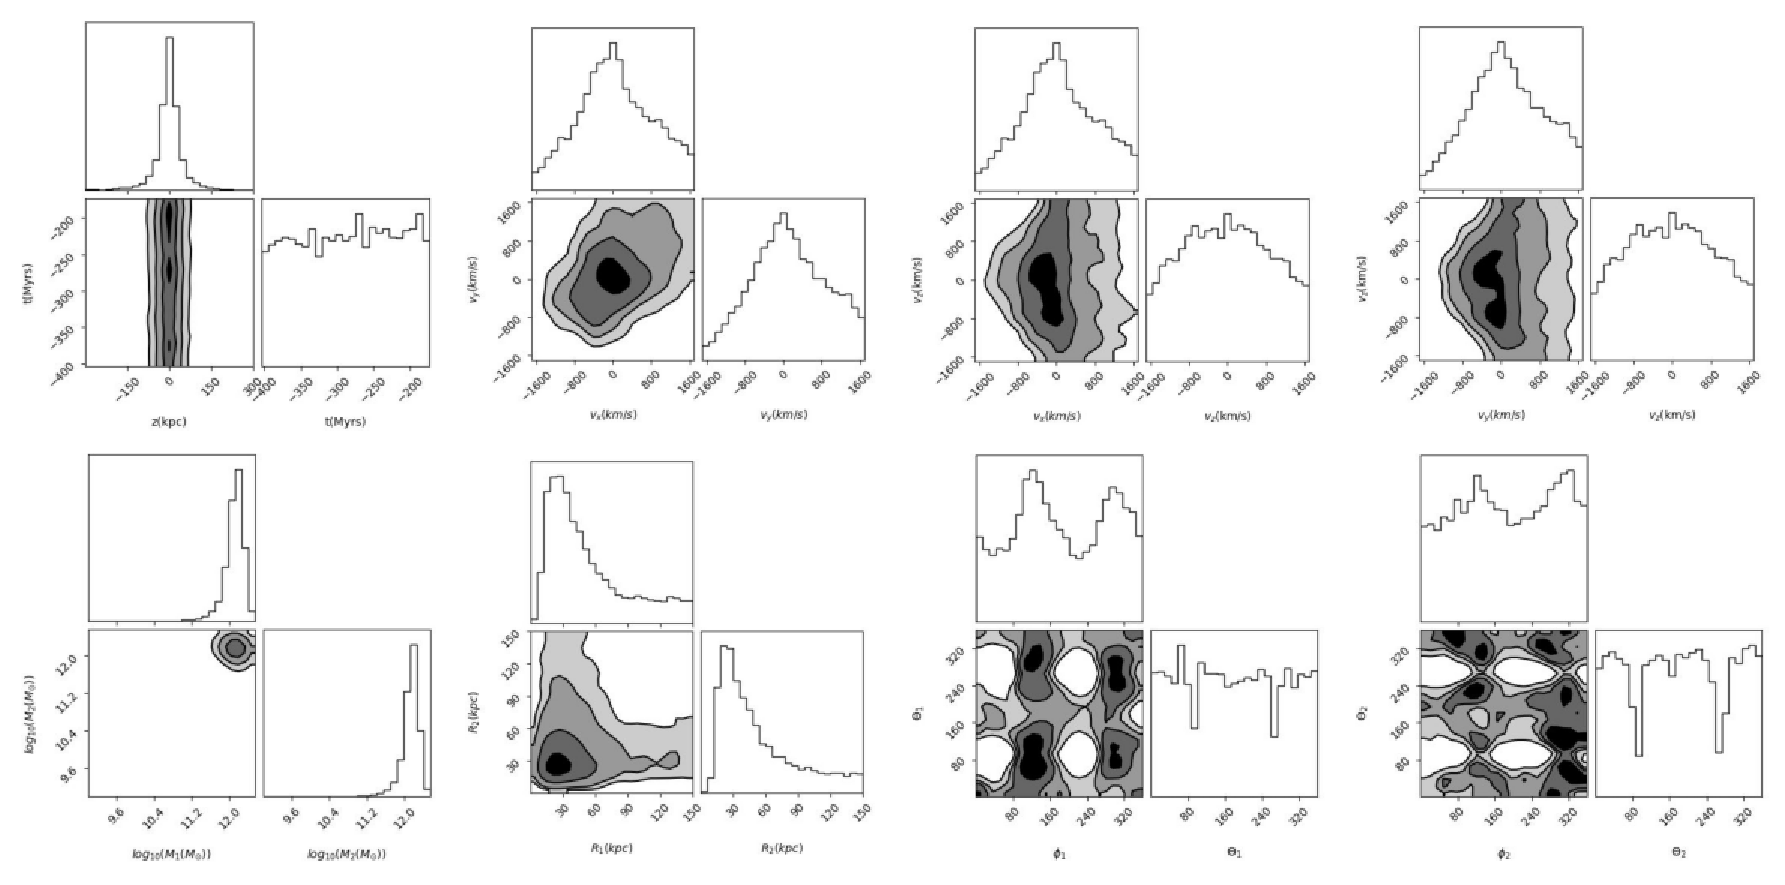
\includegraphics[width=\textwidth]{Chapter1/figures/Arp240-red-corner-obs.pdf}
    \caption{Reduced corner plot of the constraints made on the observational image of Arp 240. As shown, there is significantly more uncertainty in these measurements than those of the best fit simulation. However, we are able to make constraints on almost all parameters in the sample. The degeneracy in the orientations remains, although is less obvious in the two $\theta$ parameters. We are also unable to make conclusive constraints on the velocity parameters with the observations.}
    \label{fig:obs_corner_plot}
\end{figure*}

However, for the remainder of the parameters the level of constraint remains similar even with the change in the best fit values. We retain the two- and four-fold degeneracy in the orientation parameters. This follows on that the pipeline outright rejects disks which are edge on and loses accuracy when attempting to pin point the precise inclination of each galaxy. We are unable to make any constraint on the $\theta$ parameters, while the degeneracy of the $\phi$ parameters is still visible. The radius parameter is well constrained at 0.5$\sigma$, although with large tails in the probability space for both the primary and secondary galaxies. These tails are significantly larger here than when using the best fit simulation as the input. This is due to the observation image having no hard cutoff of the edge of the galaxy, and simply moving into more noise. The outer edges of our simulated galaxies also moves to very low signal, and therefore, there is lots of uncertainty surrounding the true radius of the galaxy. 

We retain our precise constraint on each galaxy's mass. The accuracy in the flux distribution of the primary and secondary disk is what dominates here, and therefore, we find this value incredibly quickly. The found value is comparable to the best fit simulation, although slightly lower. This is likely, again, due to the change in scale of observation. Our model uses the mass to assign flux to each particle which is then projected across the simulation. Therefore, because of the zoom in, we see that our projection of flux is significantly larger than in the best fit simulation. This means that for the same mass, are galaxy will appear larger in size. So, to maintain the correct galactic size the mass must be reduced. 

We see the same general trends when looking at the Arp 172 and Arp 290 systems. In each system, the best fit simulation scale used in GZM is much larger than the measured scale from the SDSS observations. We therefore end up with similar constraints to the different parameters, however with significant variation in the spatial parameters. The uncertainties in the radius parameters are significantly increased, while the constraint on the $\theta$ parameters is completely lost. In fact, for the same number of steps compared to constraining the best fit parameters, our MCMC fails the Geweke diagnostic. Therefore, due to the added noise running longer chains is imperative which drives up computational expense.

For the all three systems, the size of the observational image was at the limits of the simulation resolution. One simulation unit is equivalent to 15kpc. Therefore, having the image itself only be seven simulation units across would give non-physical results of the final system. Therefore, when making constraints, the observational image was artificially scaled up. We elected to scale it up by four times. This allowed us to recreate the tidal features and match the flux distribution, however, the effect this has on the mass measurements could be severe if made too large. When looking at the constraints on position here, we accounted for the scaling up by dividing the results back down. 

This leads us onto the limitations of this process to constraining galaxy interaction. While it has been very successful for many of the underlying parameters, there are many different parameters which must be provided to the pipeline so it is able to make those constraints. We discuss the limitations of applying this methodology to large interacting galaxy datasets, and how these can be offset in the short term but a long term solution is still required.

\subsection{Limitations}\label{limitations}
\noindent While this methodology does show a lot of promising in being able to constrain across populations of galaxies, it is important to note that at its base is a restricted numerical interaction code with limited resolution. There may be some interacting systems that simply cannot be modelled realistically using N-body approximations, and may therefore cause a skew in results. However, there are also some more subtle limitations which may affect how a user wishes to use this pipeline.

\subsubsection{Resolution \& Depth Effects}\label{resolution_effect}
\noindent One of the fundamental parameters that must be provided for this methodology to work is the redshift of the system. This is used to calculate the distance to the system in kpc and then converted to an assumed resolution from the known pixel scale on the sky. If this is input incorrectly the simulation images will be created at an incorrect resolution, and the MCMC will likely not reach convergence. This is also true of providing and calculating correctly an approximation of the position of the secondary galaxy. Significant computation power can be wasted if these parameters are incorrect, and will give spurious results. The reduction in resolution of the images is also a important limitation. This toy model needs small, thumbnail size images with a reasonable number of degrees of freedom as to reach convergence. Therefore, input images can only be of limited resolution which will affect the quality of the constraints we can actually make on different systems. 

The redshift is also used in scaling the fluxes calculated for each particle in the simulation. The base SED is calculated for a 1 M$_\odot$ system at a distance of 10pc. This is then scaled to the mass of the particle and then put at the distance calculated from the redshift. If the redshift is incorrect (or even slightly off) then this could lead to a bad fit for the mass of the two galaxies in the system. A flag exists in the algorithm to give it the freedom to slightly vary the redshift (and therefore the distance and resolution) by 0.001 with each step. It will then attempt to fit the redshift and resolution of the system. Note, however, this is untested and currently significantly increases computational expense.

Depth effects also play a significant role in the ability of our algorithm to fit a system. For this work, we used observations from the SDSS which is a reasonably shallow survey, being able to observe down to the 22 mag/arcsec$^{2}$. Therefore, for most of our major interacting systems, we retained the full extent of the tidal features which were created in the interaction and could provide better fitting. Our algorithm will preform significantly better when being run on systems where the clarity of the tidal features has not been lost, such as Arp 240. However, for systems that lie closer to the low surface brightness regime, our algorithm will become less efficient and require more computational expense to make effective constraints.

This also has the opposite effect in terms of tidal features formed. For example, if a system is being fit but at the true parameters a tidal feature exists which has not been detected due to its low surface brightness then our MCMC pipeline will not be able to converge on the true values. The algorithm would instead converge on those parameters where the disks were at the correct flux rather than getting the tidal features correct. Therefore, when exploring the parameter space of interacting systems with our pipeline, it is imperative that the full structure is within detection of the observing instrument.

There must be a trade off between the resolution of our simulation and the observations. In this work, we binned all of the observations down from their native pixel scale to cutouts of 100 $\times$ 100 pixels. This was so that we could still get consistent system outputs from our simulations using only 2500 particles. If lots of pixels are used, then using a low number of particles can lead to many `unphysical' output simulations. I.e. these are simulation systems where the disks will have large holes in them where there haven't been enough particles to fill the disk. To mitigate the effect of potentially using low particle numbers, we distribute the flux as described in Section \ref{flux_dist}, which is an imperfect solution. It is recommended for any user to make a balanced trade off between resolution and computational expense.

\subsubsection{Computational Expense}\label{computational_expense}
\noindent The main drawback of this methodology is that of computational expense required to run such an MCMC over a the full parameter space. In the case of this work, the simulation was set up with 2500 particles on a High End Computer Cluster with 40 CPUS. Each simulation took approximately two seconds, with the full sample run taking approximately 30 days to complete. Each galaxy was given 600 walkers to move through parameter space with each walker moving 7,500 steps. The highest memory requirement of any system was 6GB. Therefore, the runtime is very high but the memory required for it is approximately 125MB per core, therefore being very cheap in the memory.

This methodology was successful in reproducing the results of GZMs methodology - a project which took months to complete. We have automated this, and reduced the runtime required of it to 30 days on a powerful High End Computer Cluster. However, this is not the solution to the large scale dataset problems that we will be seeing when LSST comes online. If we are to run this methodology on a much larger galaxy sample - such as thousands of galaxies - then we will need to find ways to significantly improve the runtime of this method.

\section{CONCLUSIONS \& FUTURE WORK}\label{Conclusions}
\noindent In this work we have introduced an updated version of the restricted numerical simulation JSPAM and modified it to calculate and match the flux distribution of interacting galaxies based on fourteen underlying parameters. This updated algorithm, APySPAM, calculates the flux distribution by assigning particles with a Spectral Energy Distribution and accounting for star formation throughout the interaction. To test our simulation, we utilised the archived Galaxy Zoo: Mergers project, which had constrained a sample of sixty two interacting systems. In Galaxy Zoo: Mergers, volunteers used visual inspection to find the best fit simulation for observed interacting systems using the mass distribution. We have introduced a Markov-Chain Monte Carlo pipeline to directly compare simulations to observations. By relating the likelihood that a set of underlying parameters describes an observed system to the $\chi^{2}$ between that image and the simulated flux distribution we have provided a methodology to automatically put constraints on these parameters.

Using this methodology, we have found that we can constraint the best fit simulation parameters from Galaxy Zoo: Mergers to within 2$\sigma$. Every parameter of our fourteen was recoverable, however there was significant degeneracy in the orientation angles of the two galactic disks. This was expected as works such as \citet{Smith_10} found significant degeneracy between systems, but not a direct cause. In this work we find it is that, without taking account of kinematic information, multiple orientation angles can recreate observed tidal features as well as limitations in the pixel matching method of constraint. When tested on our best fit observed systems, were able to retain the excellent constraints on eight of the fourteen parameters, losing any constraint on the orientations, the z-position and the velocity parameters. However, we were able to maintain a tight constraint on the masses of the two systems. This loss of constraint was due to a loss in the signal in the tidal features/edges of the two interacting galaxies; particularly in the secondary galaxy. Therefore, deep observations of interacting systems are crucial for our methodology to work. 

There are numerous limitations to this method that any users must be aware of. First, the core simulation of this process is a restricted N-body code with a highly optimised flux distribution calculation and approximation. It is not impossible that there are systems that this pipeline can not constrain, or may give nonphysical results for. The required reduction in the parameter space of the images, such as reducing the degrees of freedom and limiting individual pixel resolution in favour of computation time, also may lead to constraints only on the disks of the galaxies and not the tidal features themselves. There is also limited time and spatial resolution within the simulation itself. When using true observations, they had to be artificially scaled up so our simulation could maintain the resolution to have constraint. In terms of the temporal and spatial parameters, this scale up can be accounted for. However, in terms of the masses of the flux distribution, this can be significantly hindered. Therefore, a user must be careful when choosing the image scales to use when attempting to constrain individual systems. 

We have demonstrated the power of this methodology and how it could be used to serve the field as large scale surveys - such as LSST - come online. Large scale automation where we can constrain interaction, make diagnostics and estimates about parameter space are not only important for inferences about individual datasets but for the interacting galaxy population as a whole. The main limitation of this method is the computational expense of it. To run this on sixty two systems, the total run time was thirty days; an unusable timescale when we are talking about interacting galaxy samples in the thousands. Therefore, future works with this algorithm and methodology will be focused on increased computational efficiency and working on larger interacting galaxy datasets. The bottleneck for computational efficiency lies in the time spent running the APySPAM simulation. While incredibly cheap individually, this is exceptionally expensive when having to be run in an MCMC chain. With the growing power of GPUs, and their ability to run numerical simulations significantly more efficiently than CPUs, one solution may already exist. This, combined with further developments in methodologies such as simulation based inference, machine learning and Gaussian processes could begin to reduce computation time.

%\section*{ACKNOWLEDGEMENTS}
% Will be re-written after getting some advice of what to write.

% \bibliographystyle{mnras}
% \bibliography{Paper_1_References}